\chapter{Analiza jakości dopasowania śladów w oparciu o test $\chi^2$}
\section{Selekcja przypadków}
W celu wykonania analizy jakości dopasowania śladów posłużono się rozpadem 
\begin{equation}
B_d \rightarrow J/\Psi(\rightarrow \mu +\mu) + K_s(\rightarrow \pi + \pi )
\end{equation}

Jest to rozpad pół leptonowy, który da się opisać przy użyciu diagramu Feynmana zamieszczonego na rysunku \ref{rys:BJPsi}.

 \begin{figure}[h]
 \centering
 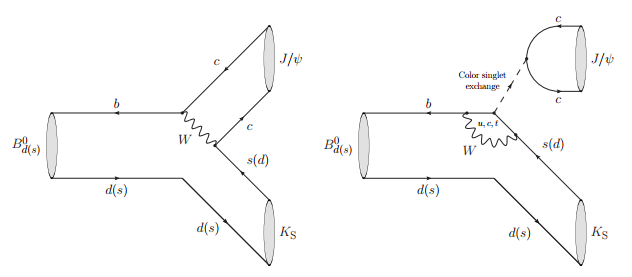
\includegraphics[scale=0.8]{rozdzial6/Feynman.png}
 % GAUDI.jpeg: 767x379 pixel, 96dpi, 20.29x10.03 cm, bb=0 0 575 284
 \caption{Diagramy Feynmana obrazujące topologię rozpadu $B_d \rightarrow J/\Psi(\rightarrow \mu +\mu) + K_s(\rightarrow \pi + \pi )$. po lewej diagram typu drzewiastego, po prawej typu pingwin. }
 \label{rys:BJPsi}
\end{figure}

Faktem, wartym podkreślenia jest, że w podczas analizy wzięto pod uwagę przypadki w których z produktami rozpadów mezonu $K_s$, czyli pionami, stowarzyszono ślady zarówno długie jak i typu "Downstream".
\section{Analiza bazująca an symulacjach Monte Carlo} 
Ten podrozdział zawiera wyniku uzyskane dla symulowanych danych Monte Carlo. 
W dalszej części pracy przyjęte zostanie oznaczenie:
\begin{equation}
\chi^2 \equiv \frac{\chi^2}{\nu} 
\end{equation}

\subsection{Wydajność rekonstrukcji śladów}
Pierwszym elementem pracy w analizie jakości dopasowania śladów w eksperymencie LHCb jest zbadanie wydajności rekonstrukcji śladów. Jest to bardzo istotna analiza, która w bardzo szybko sposób obrazuje jaki ułamek rekonstruowanych śladów jest związany z interesującym rozpadem. Z praktycznego punktu widzenia wydajność (ang. efficiency) jest wyliczana przy wykorzystaniu informacji dotyczącej numeru pdg cząstki \cite{PDG}. natomiast formalna, matematyczna definicja jest realizowana przy użyciu zależności:

\begin{eqnarray}
\varepsilon &=& \frac{\# sladów\_jezeli\_nr\_pdg\_rodzica\_jest\_odpowiedni }{\# wszystkich\_sladów} \\ \nonumber &=&\frac{a_{total}}{n_{total}}
\end{eqnarray}
Natomiast niepewność wyznaczenia tej wielkości przyjmuje się jako:
\begin{equation}
\sigma_{\varepsilon}=\frac{\sqrt{a_{total}(1-\varepsilon)}}{n_{total}}
\end{equation}

\begin{figure}[H]
\centering
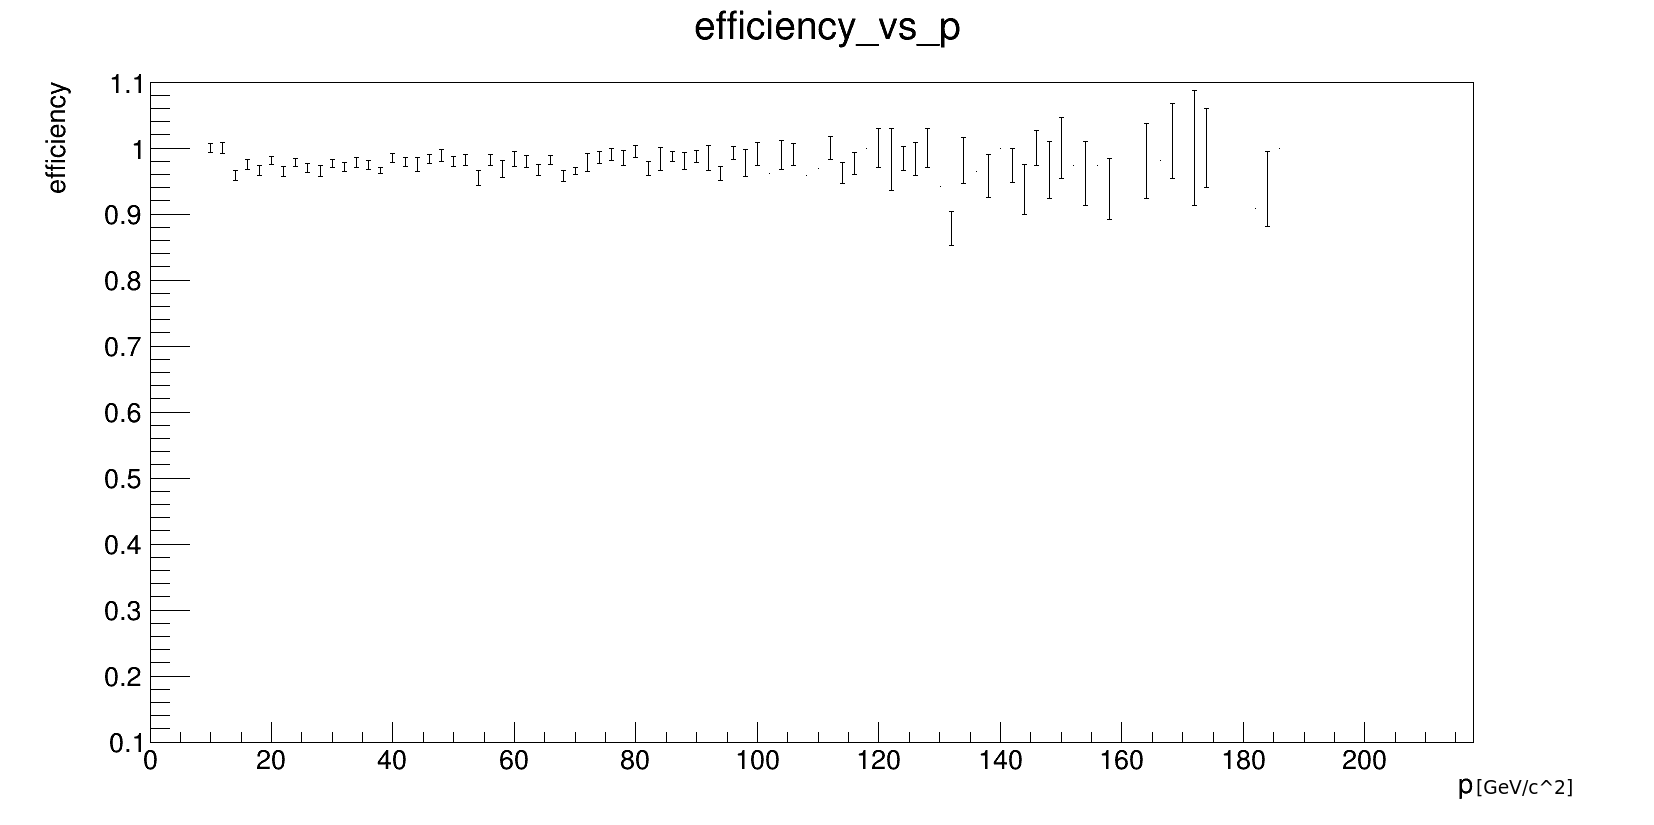
\includegraphics[scale=0.3]{rozdzial6/Jpsi_p.png} \\
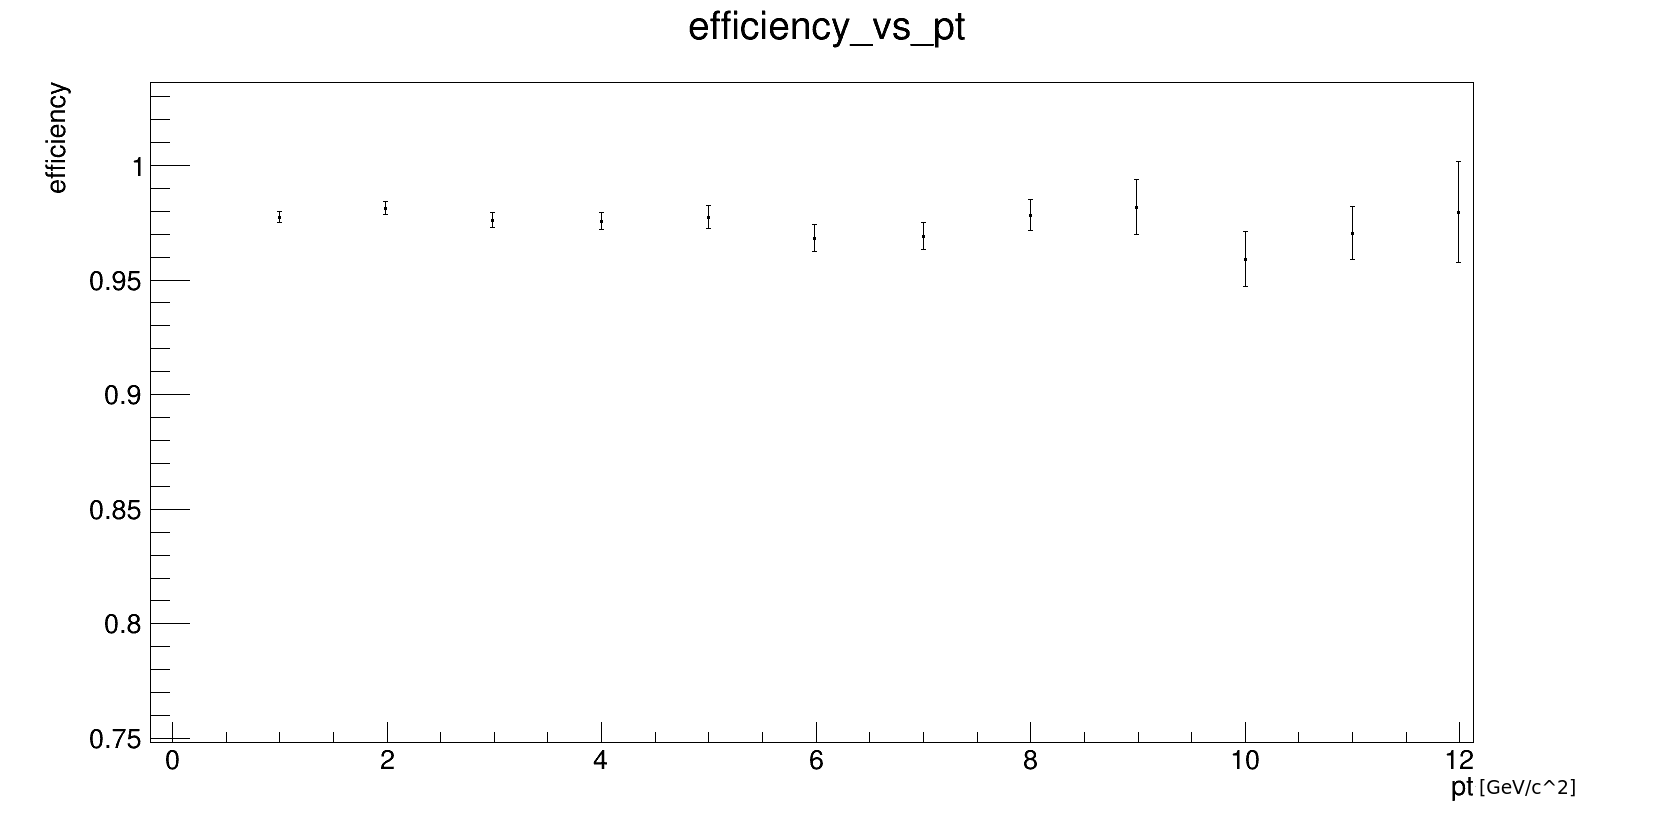
\includegraphics[scale=0.3]{rozdzial6/Jpsi_pt.png} \\
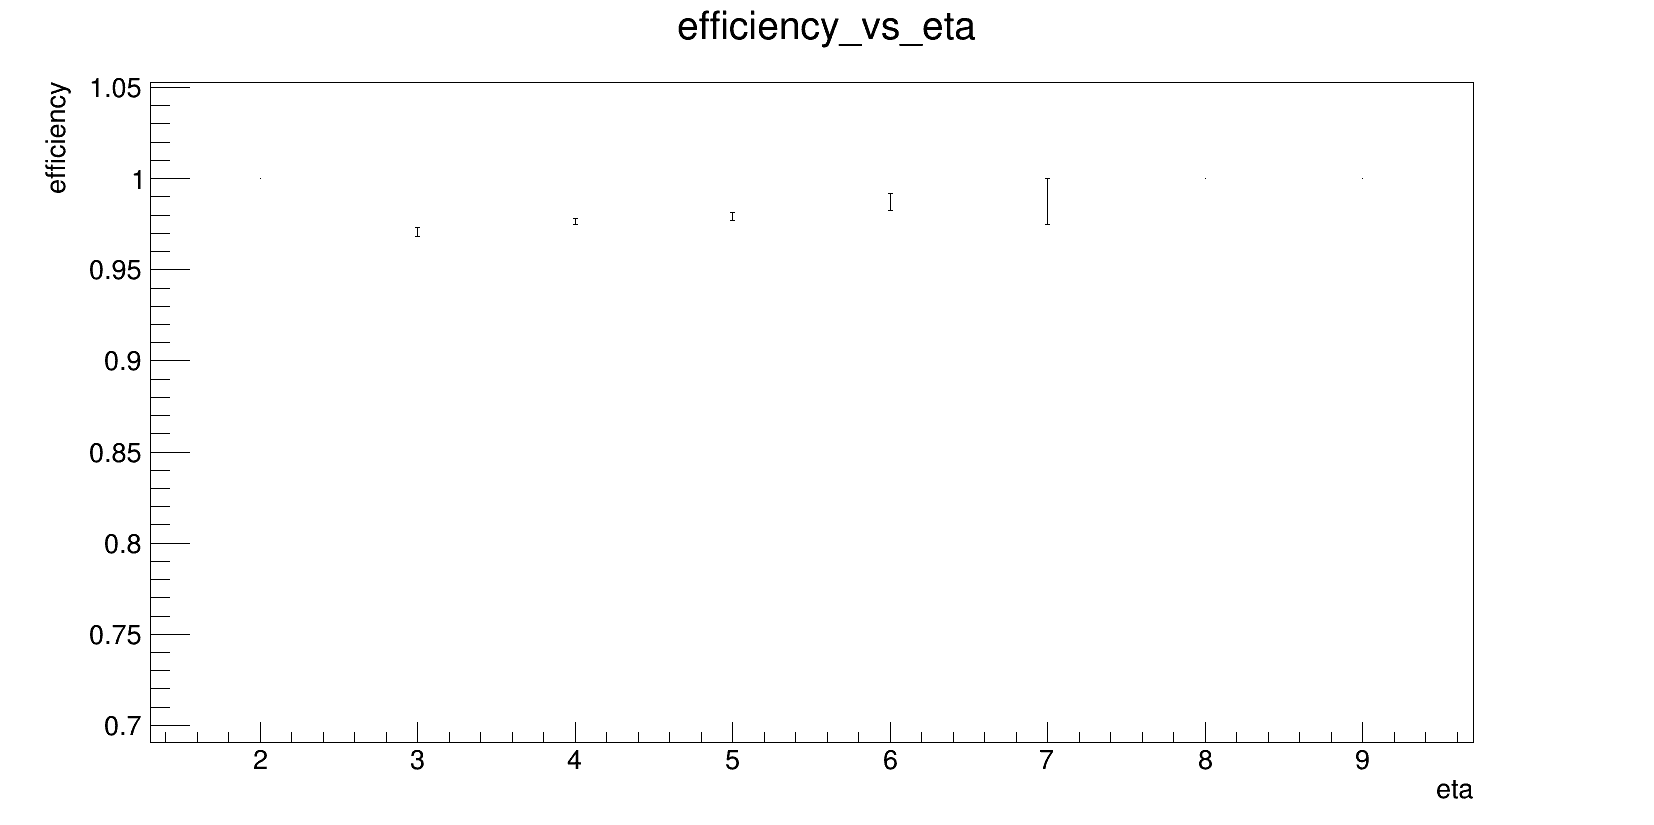
\includegraphics[scale=0.3]{rozdzial6/Jpsi_eta.png} \\ 
\caption{Wydajność rekonstrukcji śladów długich zrekonstruowanych dla cząstek z rozpadu $J/\Psi \rightarrow \mu + \mu $  w funkcji pędu (góra), pędu poprzecznego (środek) oraz pseudorapidity (dół).}
\label{effJPsi}
\end{figure}



\begin{figure}[H]
\centering
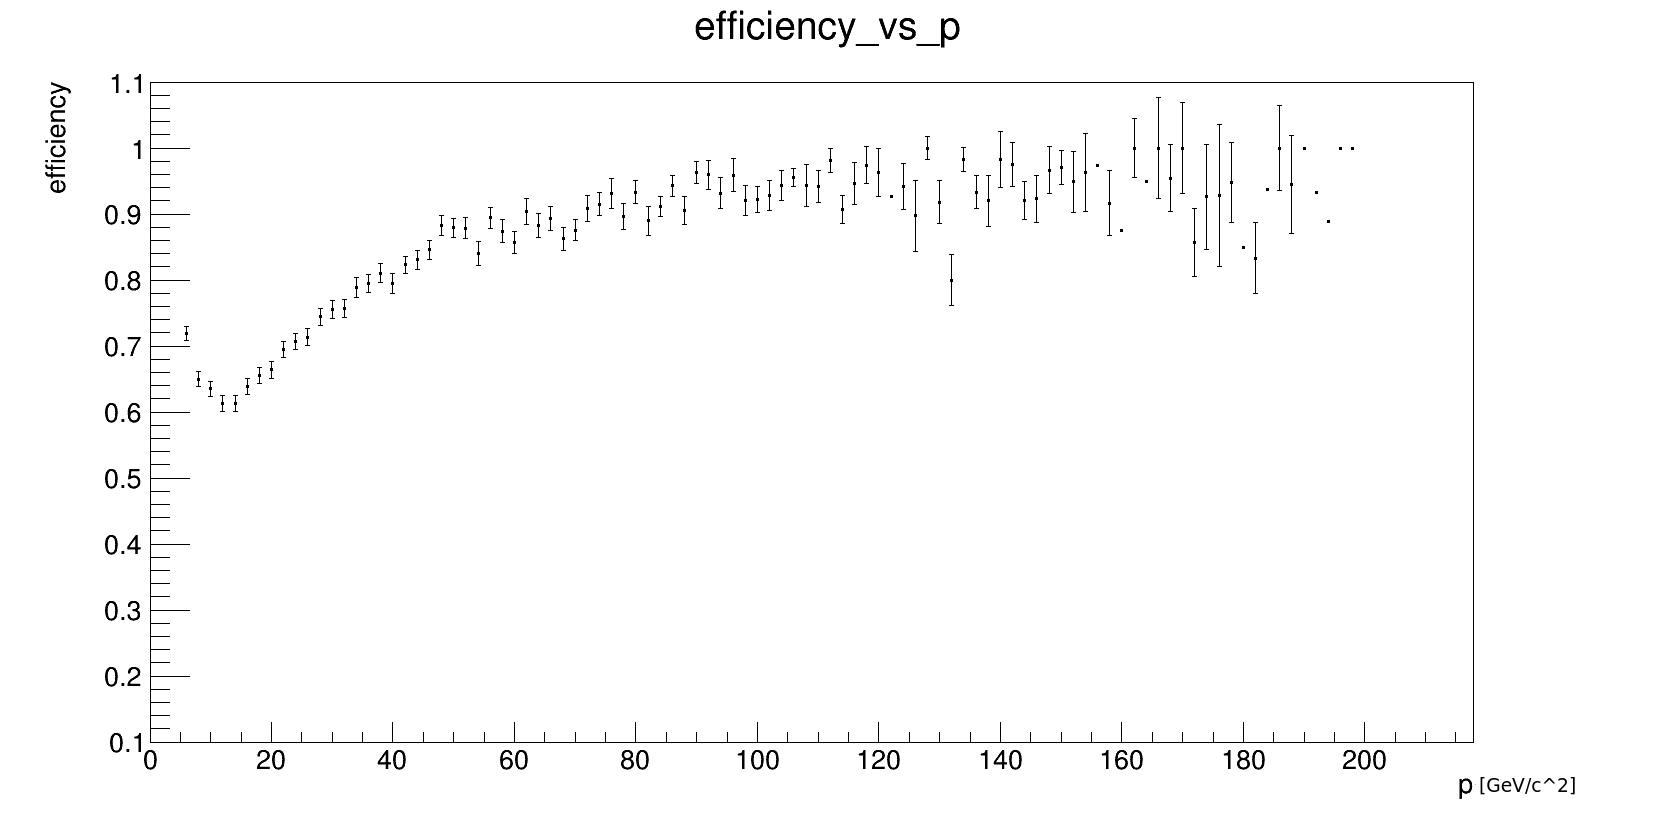
\includegraphics[scale=0.3]{rozdzial6/KsLL_p.png} \\
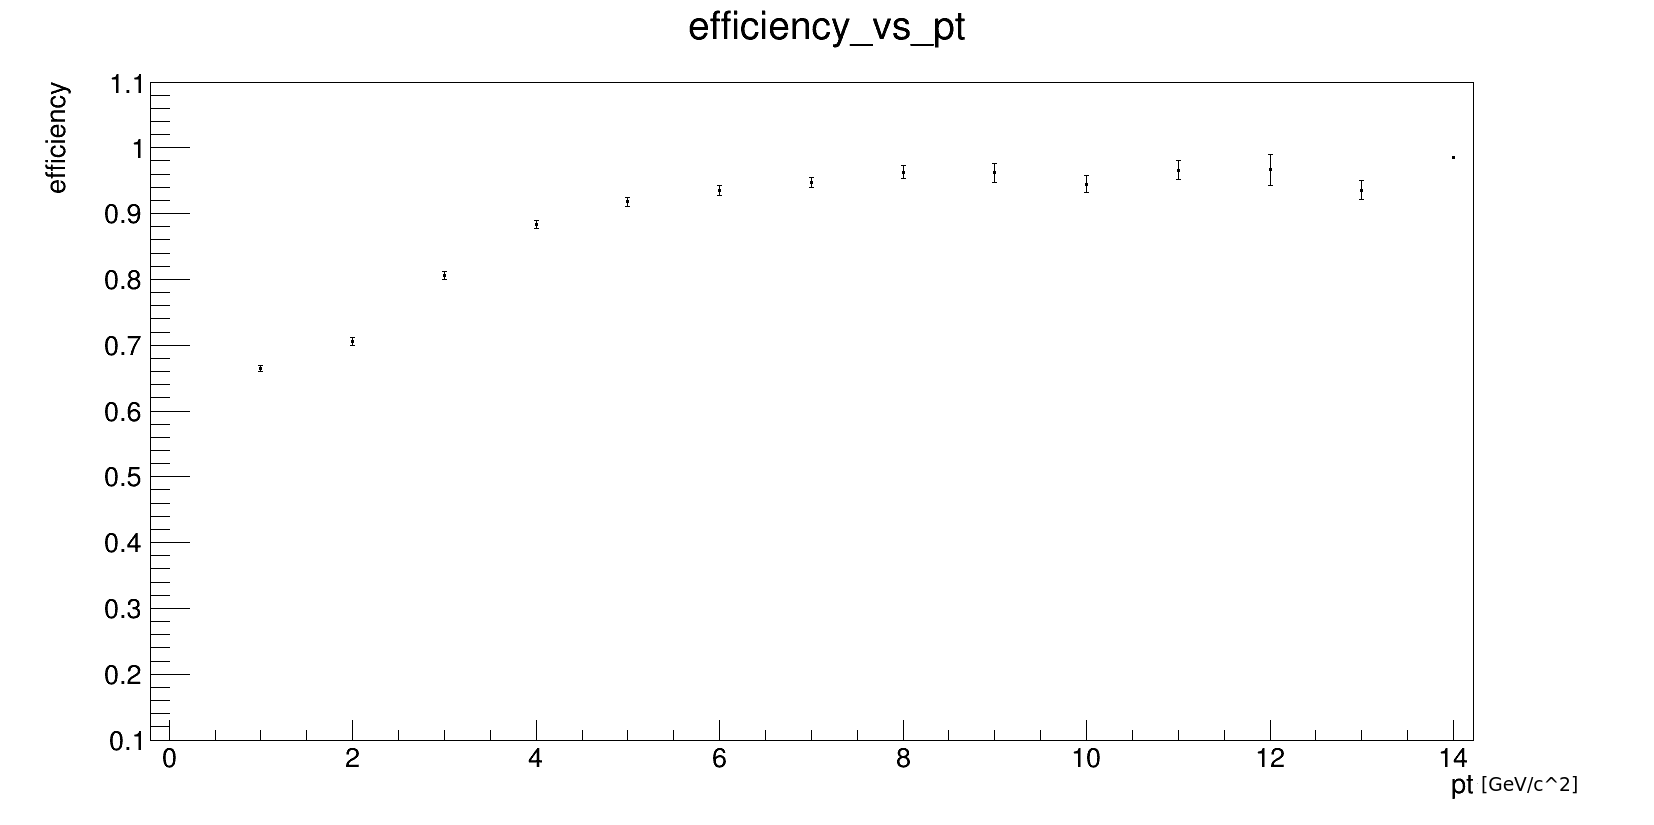
\includegraphics[scale=0.3]{rozdzial6/KsLL_pt.png} \\
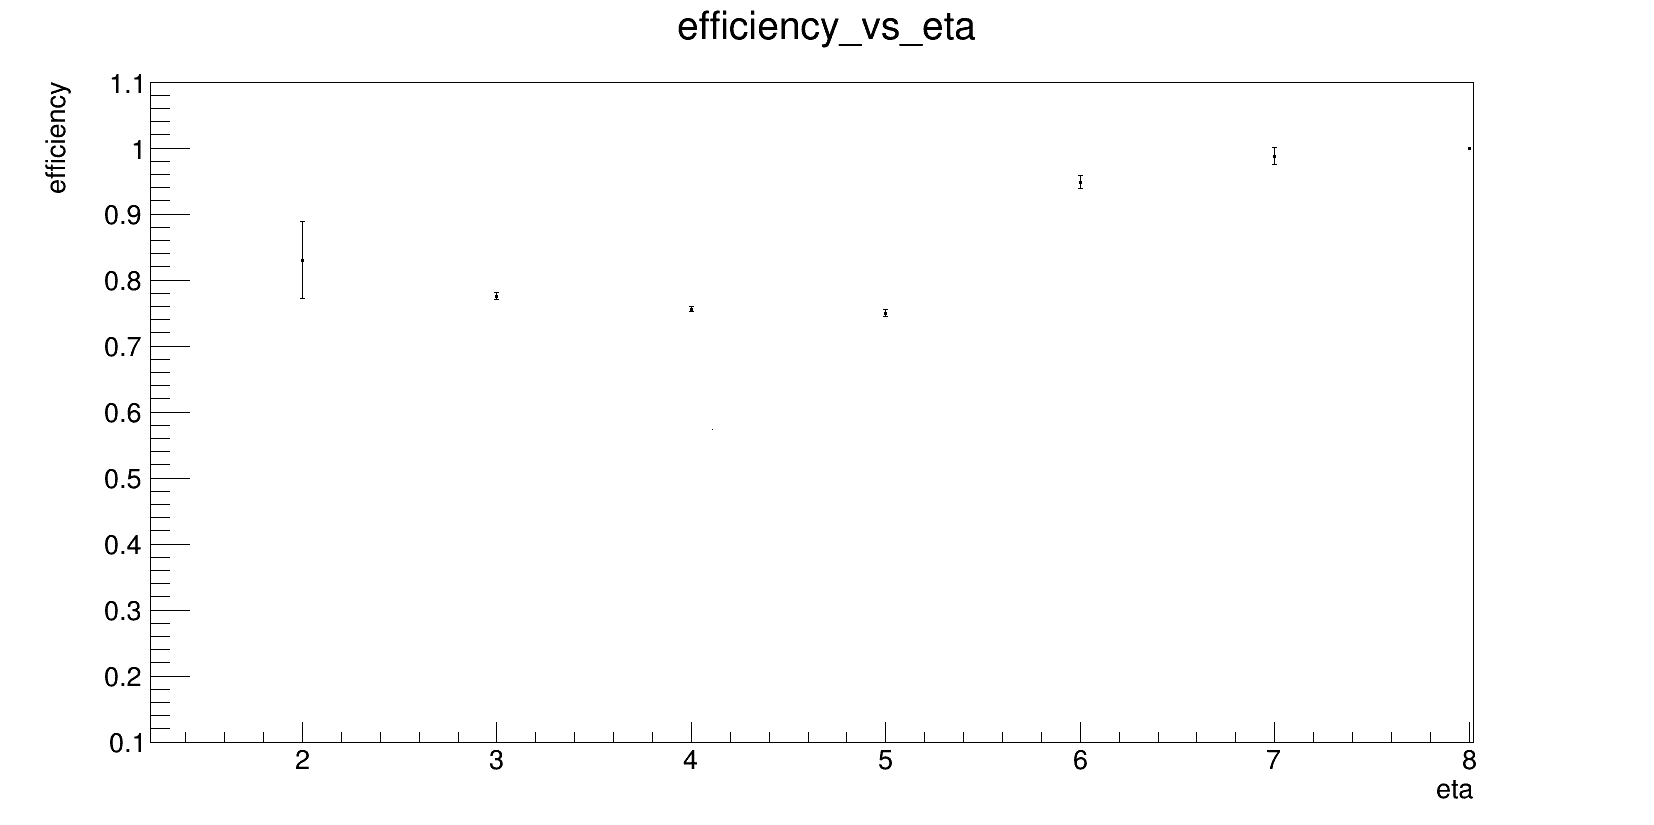
\includegraphics[scale=0.3]{rozdzial6/KsLL_eta.png} \\ 
\caption{Wydajność rekonstrukcji śladów \textbf{długich} zrekonstruowanych dla cząstek z rozpadu $K_s \rightarrow \pi + \pi $  w funkcji pędu (góra), pędu poprzecznego (środek) oraz pseudorapidity (dół).}
\label{KsLL}
\end{figure}

\begin{figure}[H]
\centering
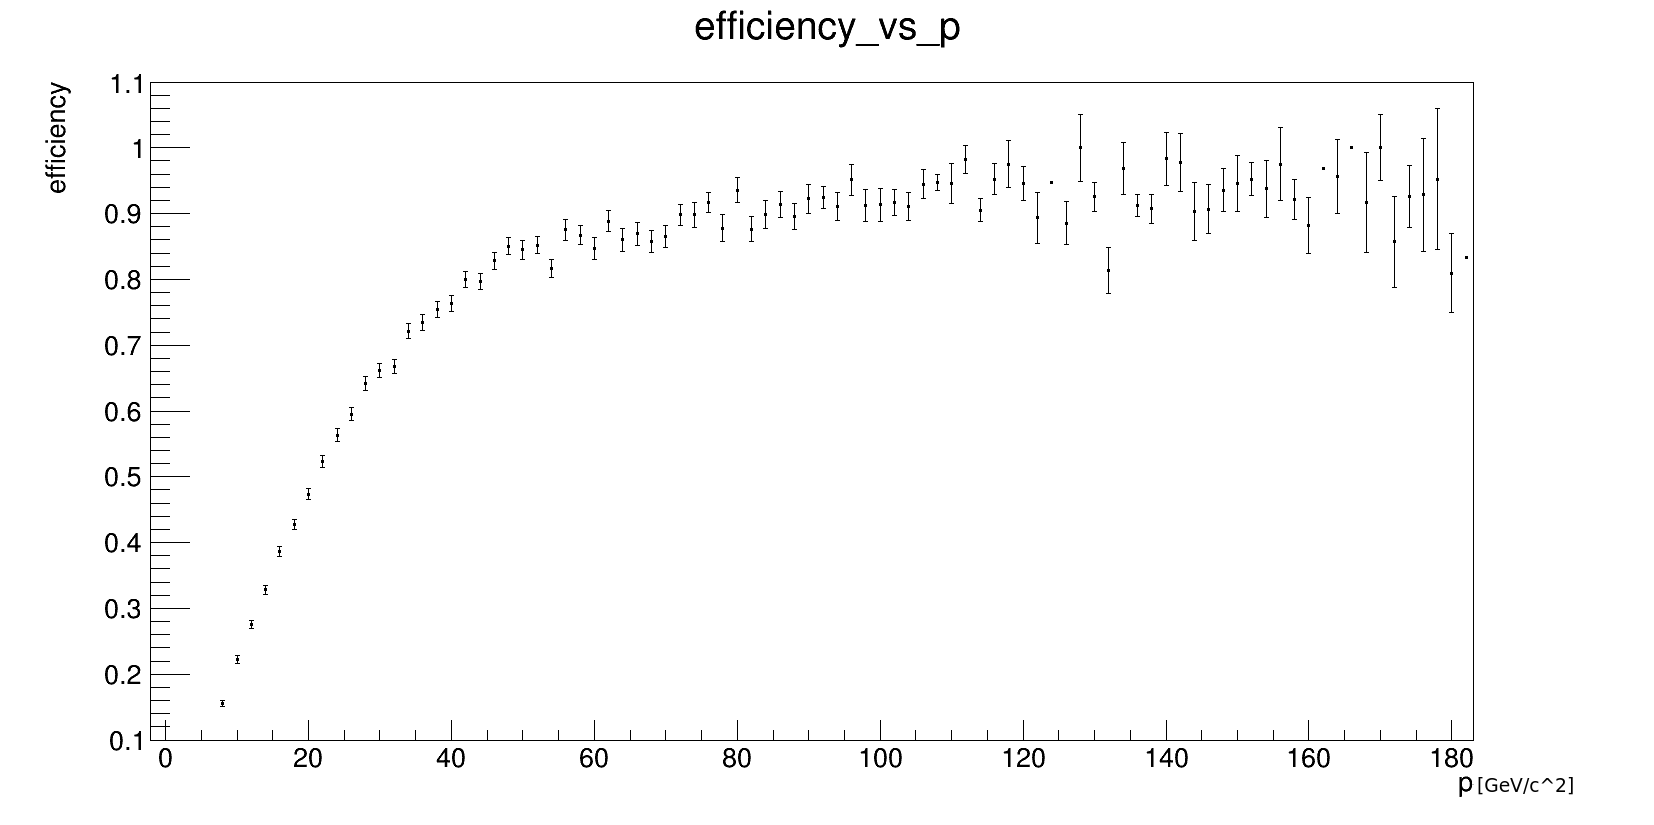
\includegraphics[scale=0.25]{rozdzial6/KsDD_p.png} \\
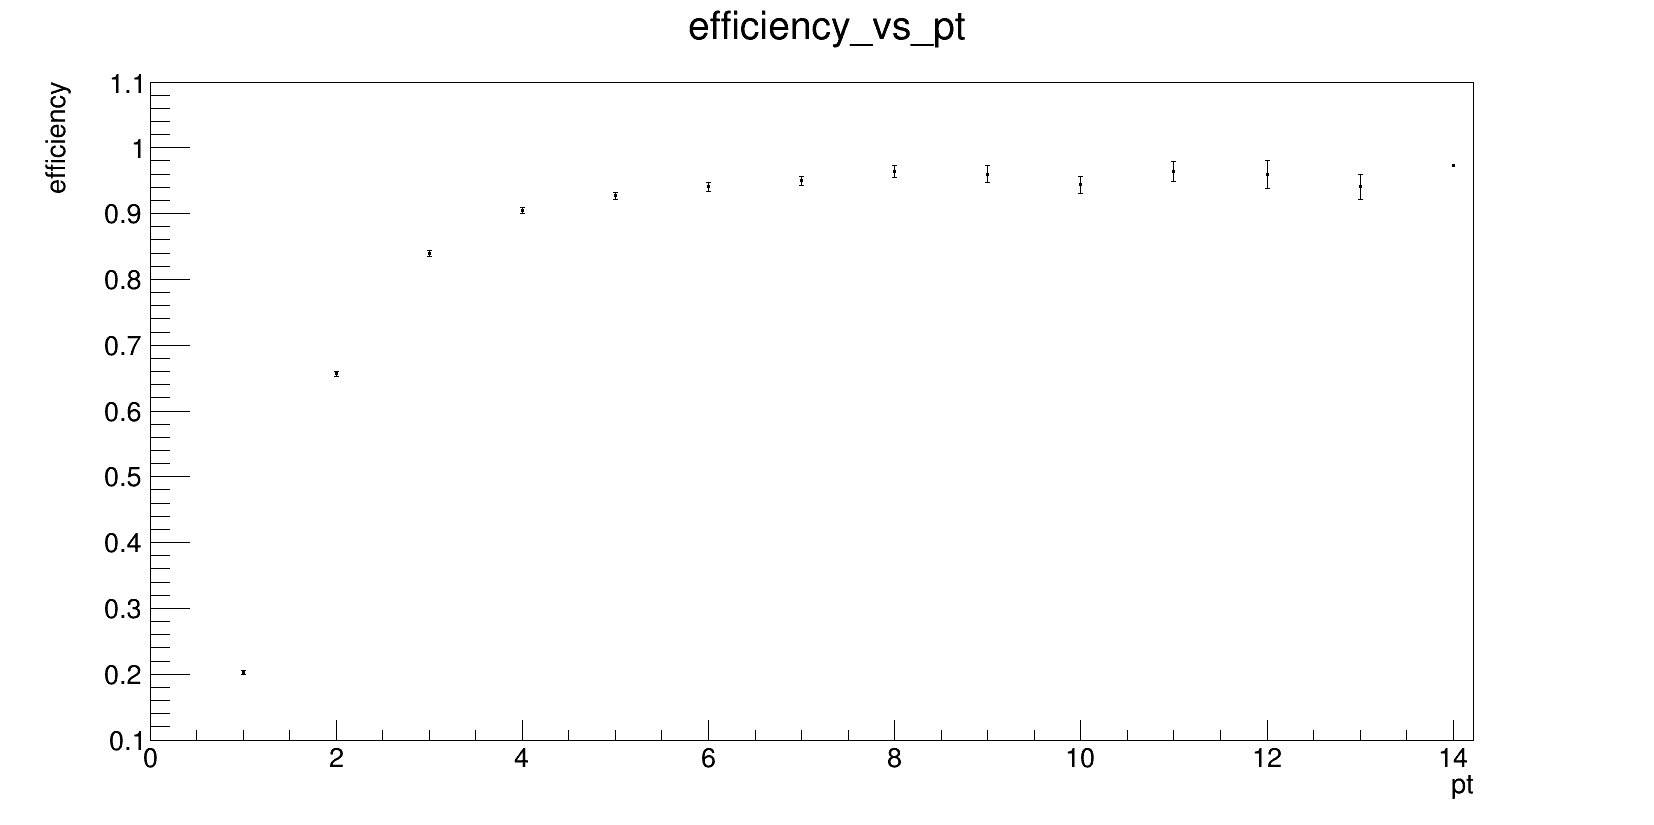
\includegraphics[scale=0.25]{rozdzial6/KsDD_pt.png} \\
\caption{Wydajność rekonstrukcji śladów \textbf{typu downstream} zrekonstruowanych dla cząstek z rozpadu $K_s \rightarrow \pi + \pi $  w funkcji pędu (góra), pędu poprzecznego (dół).}
\label{KsDD}
\end{figure}

Na rysunku \ref{effJPsi} przedstawiono zależności wydajności rekonstrukcji śladów długich pochodzących z rozpadu mezony $J\/ \Psi$.  Nie zauważono żadnych korelacji pomiędzy wartością parametrów pędu, pędu poprzecznego oraz pseudorapidity. Warto zwrócić uwagę na bardzo dobrą jakość rekonstrukcji śladów nawet dla małych wartości pędu, zarówno całkowitego jak i poprzecznego. W porównaniu do do rysunku \ref{effJPsi} sytuacja dla śladów stowarzyszonych z rozpadem mezonu $K_s \rightarrow \pi + \pi $ zarówno dla śladów długich jak i typu "downstream" jest inna. Wyraźnie widać zależność od pędu, dla małych jego wartości wydajność rekonstrukcji jest dość niska. Dopiero dla wartości pędu całkowitego większych od $40GeV/c^2$ rozkłady są praktycznie identyczne. 

Warto również przypatrzeć się niepewnością wyznaczenia wydajności rekonstrukcji. Łatwo zauważyć, że wzrasta ona wraz ze wzrostem wartości pędów, poprzecznego i całkowitego. Efekt ten jest łatwo wyjaśnić, gdyż dla takich wartości gwałtownie spada ilość rejestrowanych cząstek.  

\subsection{Rozkłady $\chi^2$}
Następnym krokiem dokonanym w wyniku studiów nad jakością dopasowania śladów było posłużenie się testem $\chi^2$. W tym celu wygenerowano rozkłady $\chi^2$ dla każdego ze śladów. Zgodnie z tym, co opisano w rozdziale 4 $\chi^2$ jest wielkością addytywną więc można zapisać iż całkowita wartość $\chi^2_{total}$ dla śladu jest równa sumie przyczynków zrekonstruowanych w różnych detektorach. W formie matematycznej można to zapisać jako:
\begin{equation}
\chi^2_{total}=\chi^2_{Velo}+\chi^2_{T}+\chi^2_{TT}
\label{chiTotal}
\end{equation} 

\begin{figure}[H]    
\begin{minipage}[t]{0.55\textwidth}
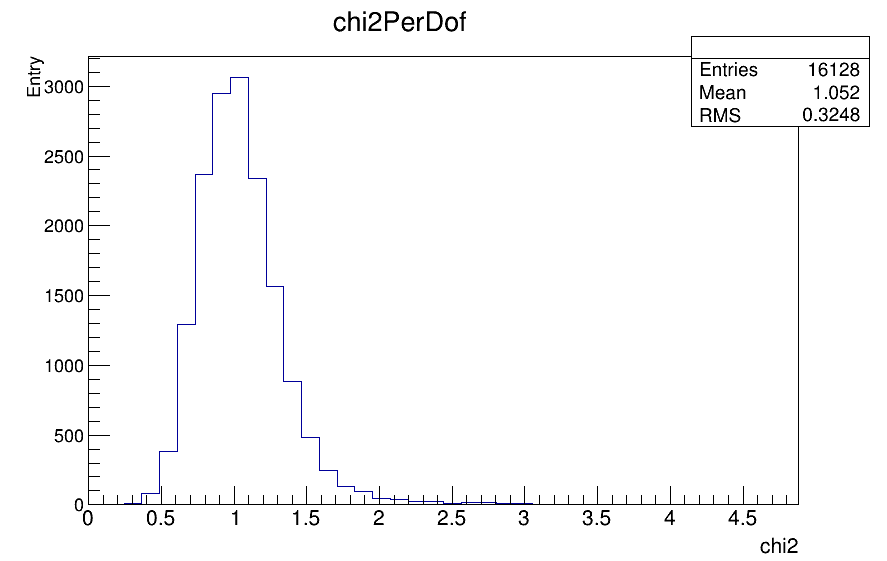
\includegraphics[width=\linewidth]{rozdzial6/JPsi_chi2.png}
\end{minipage}
\hspace{\fill}
\begin{minipage}[t]{0.55\textwidth}
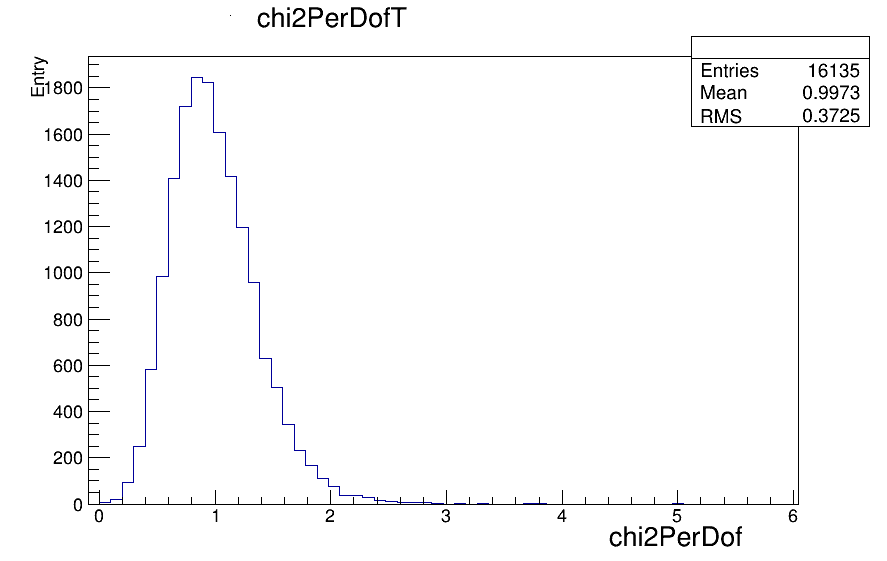
\includegraphics[width=\linewidth]{rozdzial6/JPsi_chi2T.png}
\end{minipage}

\vspace*{0.5cm} % (or whatever vertical separation you prefer)
\begin{minipage}[t]{0.55\textwidth}
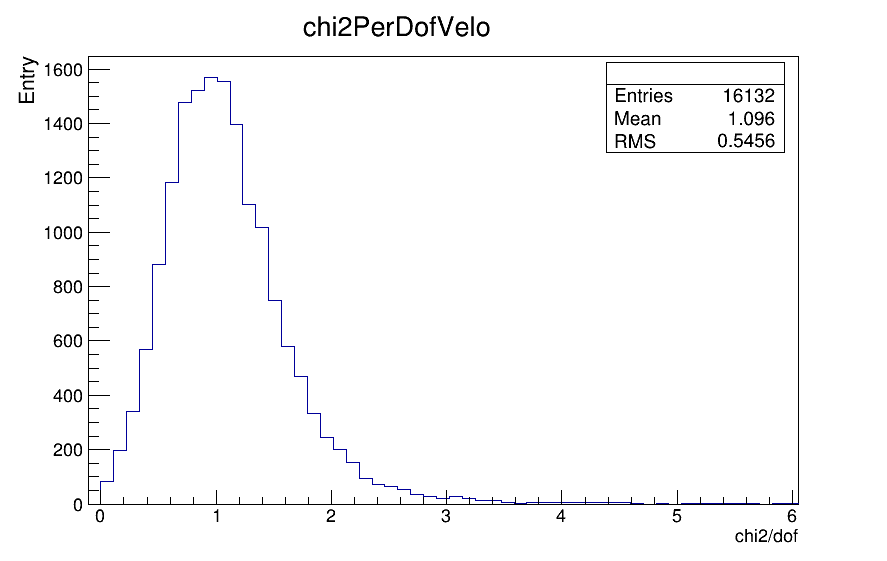
\includegraphics[width=\linewidth]{rozdzial6/JPsi_chi2Velo.png}
\end{minipage}
\hspace{\fill}
\begin{minipage}[t]{0.55\textwidth}
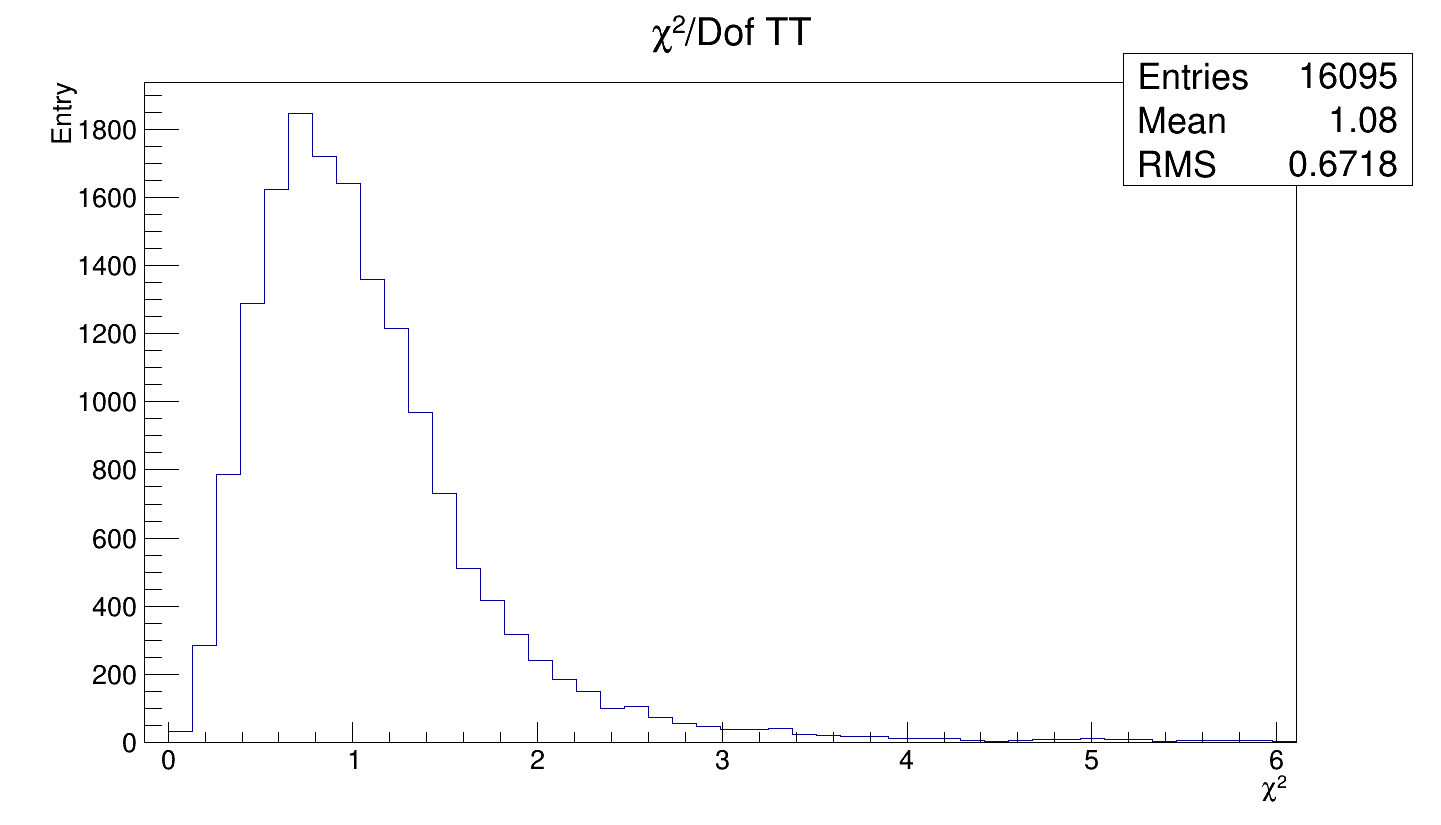
\includegraphics[width=\linewidth]{rozdzial6/JPsi_chi2TT.png}
\end{minipage}
\caption{Rozkłady $\chi^2$ wyliczone dla śladów zrekonstruowanych w wyniku oddziaływania produktów rozpadu mezonu $J/\Psi$. Na rysunku (góra lewo) przedstawiono całkowity $\chi^2$, na (góra prawo) rozkład dla części T, natomiast na dole rozkłady dla Velo (lewo) oraz TT (prawo) } \label{chi2JPsi}
\end{figure}


Rysunek \ref{chi2JPsi} przedstawia rozkłady $\chi^2$ dla wybranego śladu wytworzonego w wyniku rozpadu mezonu $J/ \Psi$.  Bardzo wyraźnie widać, że najbardziej niepokojący fragment jest ten, pochodzący pochodzący od detektora TT. Znaczna ilość przypadków jest niefizyczna, o bardzo małej, mniejszej od jednego, wartości $\chi^2$. Jak wspominano w rozdziale 4, prawdopodobna przyczyną takiego stanu rzeczy jest nieprawidłowe wyznaczenie niepewności pomiarowych. Dla potwierdzenia słuszności rozumowania na rysunkach \ref{KsDD} oraz \ref{KsLL} przedstawiono  podobne rozkłady, tym razem dla ślady są stowarzyszone z produktami rozpadu mezonu $Ks$.
\begin{figure}[h]    
\begin{minipage}[t]{0.45\textwidth}
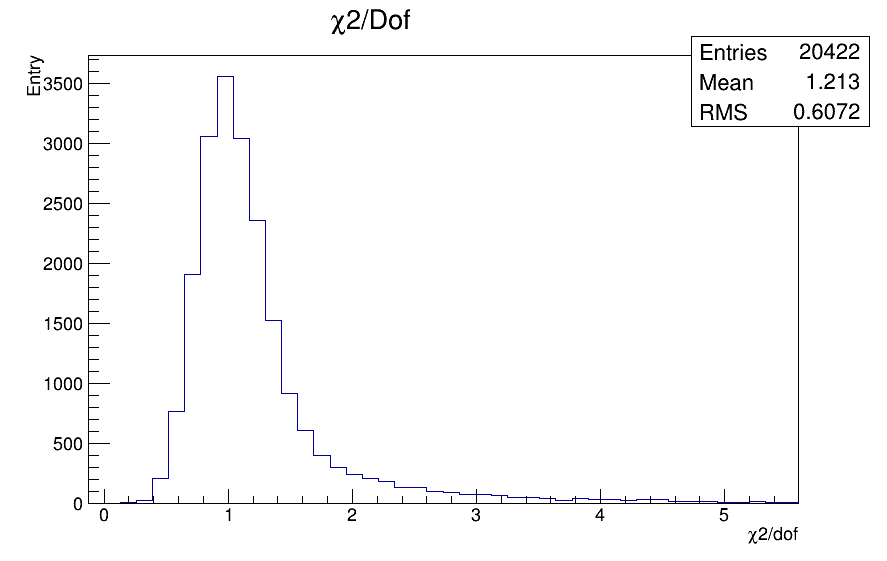
\includegraphics[width=\linewidth]{rozdzial6/KsLL_chi2.png}
\end{minipage}
\hspace{\fill}
\begin{minipage}[t]{0.45\textwidth}
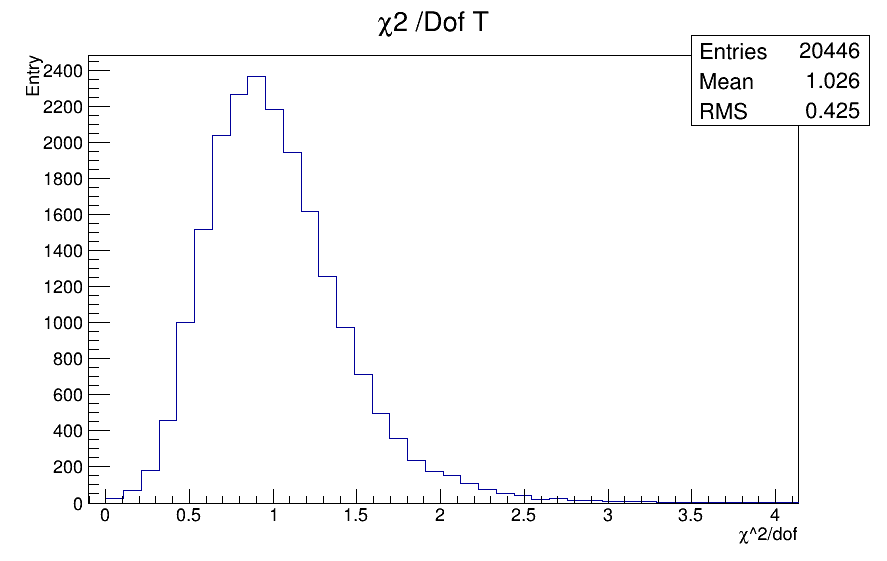
\includegraphics[width=\linewidth]{rozdzial6/KsLL_chi2T.png}
\end{minipage}

\vspace*{0.5cm} % (or whatever vertical separation you prefer)
\begin{minipage}[t]{0.45\textwidth}
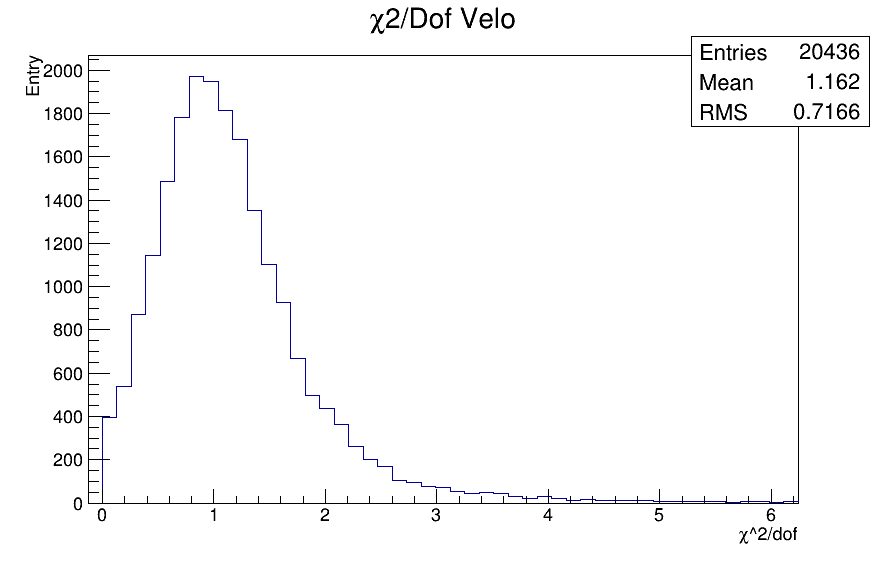
\includegraphics[width=\linewidth]{rozdzial6/KsLL_chi2Velo.png}
\end{minipage}
\hspace{\fill}
\begin{minipage}[t]{0.5\textwidth}
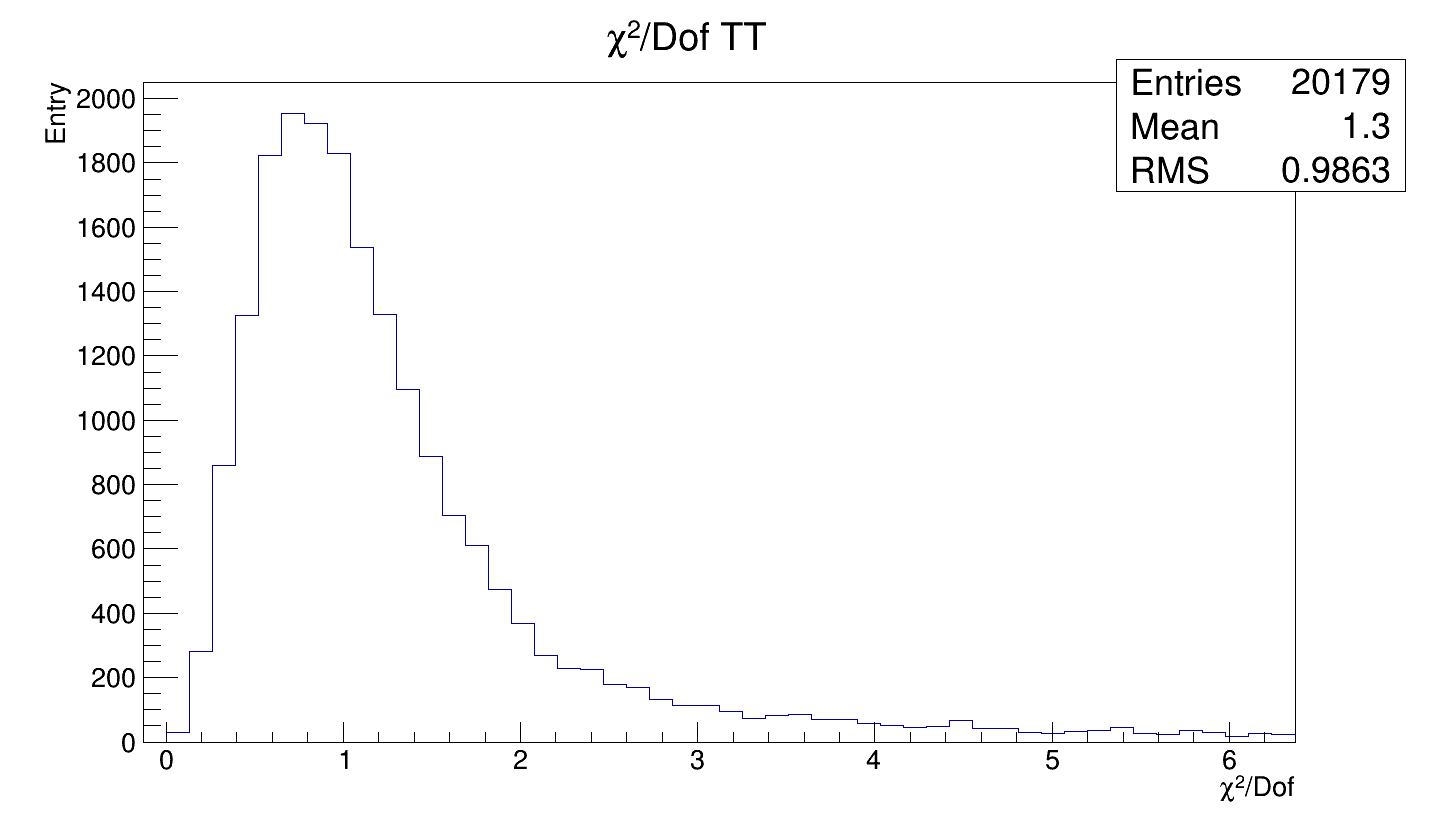
\includegraphics[width=\linewidth]{rozdzial6/KsLL_chi2TT.png}
\end{minipage}
\caption{Rozkłady $\chi^2$ wyliczone dla śladów \textbf{długich} zrekonstruowanych w wyniku oddziaływania produktów rozpadu mezonu $Ks$. Na rysunku (góra lewo) przedstawiono całkowity $\chi^2$, na (góra prawo) rozkład dla części T, natomiast na dole rozkłady dla Velo (lewo) oraz TT (prawo) } \label{chi2KsLL}
\end{figure}

\begin{figure}[H]    
\begin{minipage}[t]{0.4\textwidth}
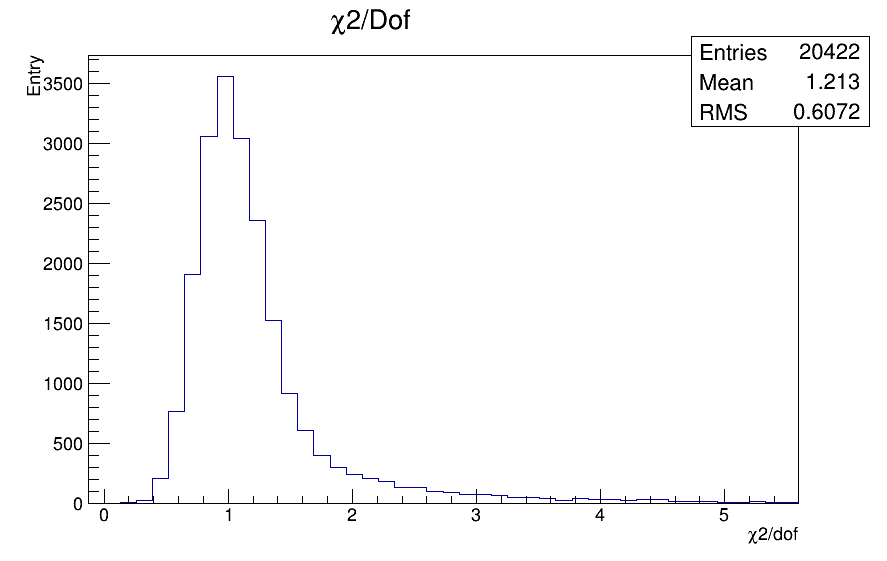
\includegraphics[width=\linewidth]{rozdzial6/KsLL_chi2.png}
\end{minipage}
\hspace{\fill}
\begin{minipage}[t]{0.4\textwidth}
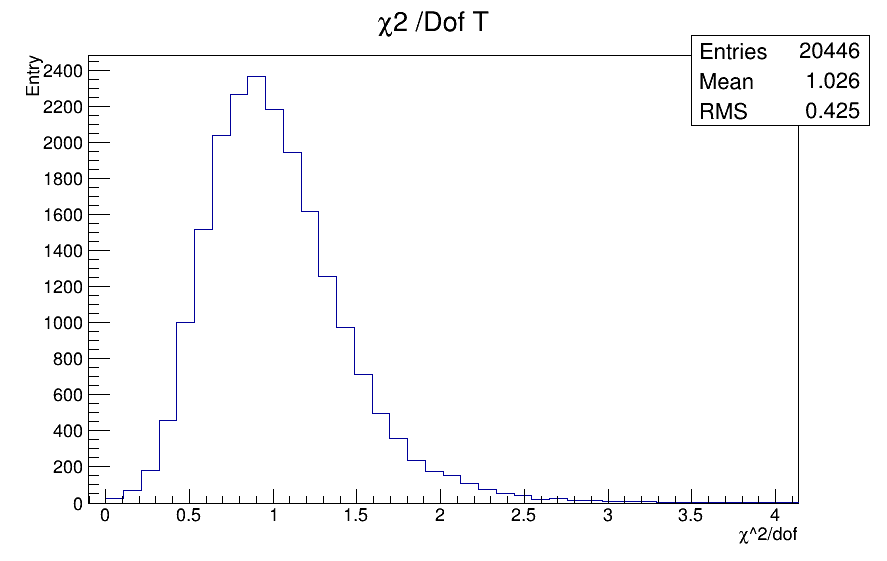
\includegraphics[width=\linewidth]{rozdzial6/KsLL_chi2T.png}
\end{minipage}

\vspace*{0.5cm} % (or whatever vertical separation you prefer)
\hspace{\fill}
\begin{minipage}[t]{\textwidth}
\centering
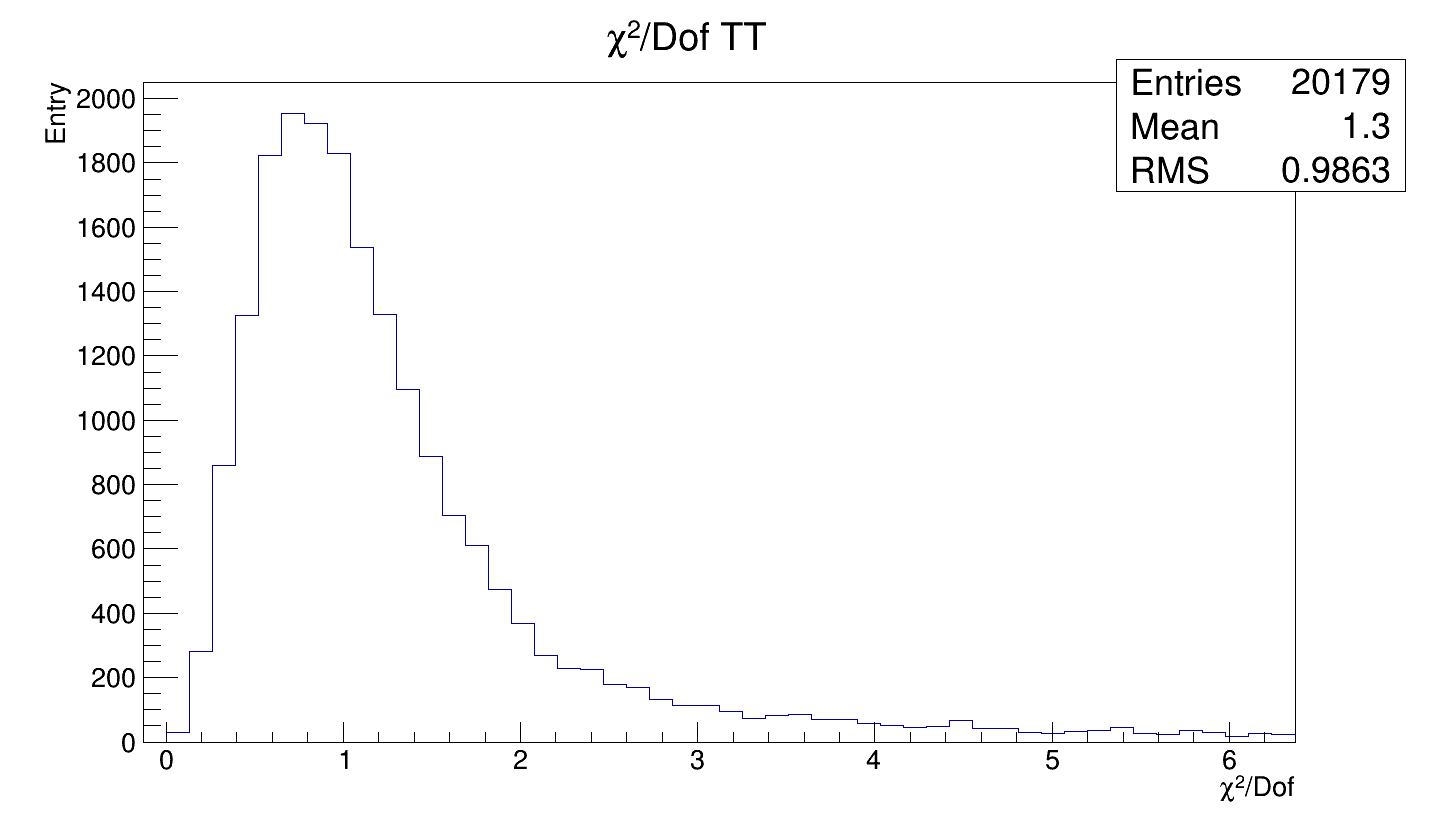
\includegraphics[scale=0.2]{rozdzial6/KsLL_chi2TT.png}
\end{minipage}
\caption{Rozkłady $\chi^2$ wyliczone dla śladów \textbf{typu downstream} zrekonstruowanych w wyniku oddziaływania produktów rozpadu mezonu $K_s$. Na rysunku (góra lewo) przedstawiono całkowity $\chi^2$, na (góra prawo) rozkład dla części T, natomiast na dole dla  TT. } \label{chi2KsDD}
\end{figure}

\subsection{Zależności korelacyjne}
Zaprezentowanie samych rozkładów $\chi^2$, będące dość interesujące z punktu widzenia analizy pozostawiałoby spory niedosyt. Dlatego bardzo istotnym krokiem w analizie było wykonanie wykresów korelacji pomiędzy otrzymanej wartości $\chi^2$ a innymi parametrami. Na serii poniższych rysunków takie  zależności korelacyjne zostały narysowane. Z racji bardzo dużej ilości rysunków w niniejszej pracy zaprezentowane, jako przykładowe, jednocześnie dobrze obrazujące wszystkie  zaobserwowane efekty, będą odpowiednie wykresy związane z śladami długimi utworzonymi przez produkty rozpadu mezonu $Ks$. Dalsza analiza tych śladów jest istotniejsza z powodu zaobserwowanych anomalii w wydajności rekonstrukcji oraz  pojawienie się znaczącej liczby niefizycznych ( o zbyt malej wartości $\chi^2$) w sektorze TT. 

\begin{figure}[H]    
\begin{minipage}[t]{0.5\textwidth}
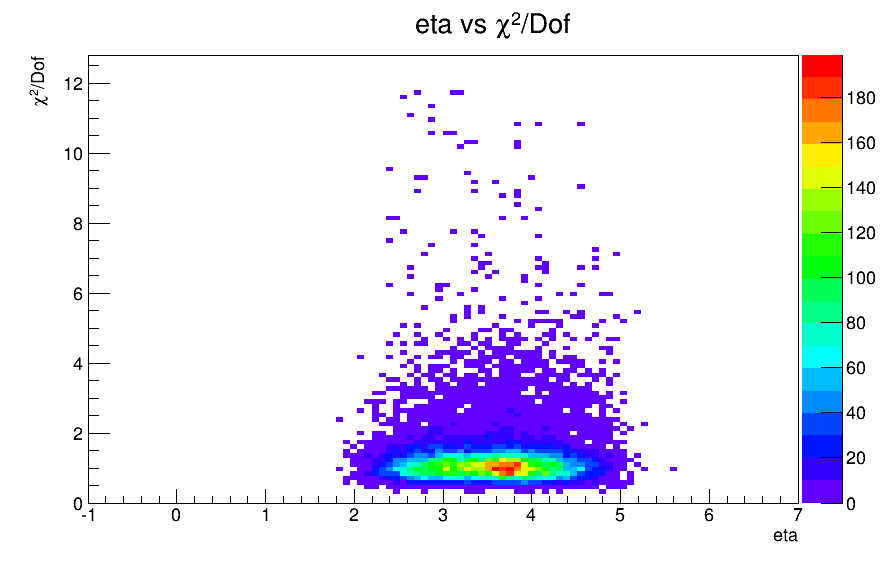
\includegraphics[width=\linewidth]{rozdzial6/JPsi_eta_chi2.png}
\end{minipage}
\hspace{\fill}
\begin{minipage}[t]{0.5\textwidth}
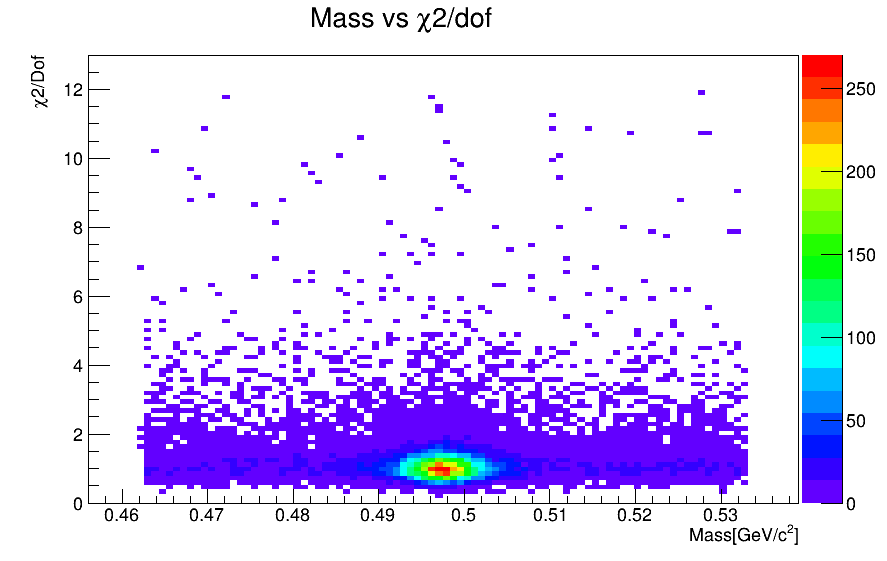
\includegraphics[width=\linewidth]{rozdzial6/JPsi_mass_chi2.png}
\end{minipage}

\vspace*{0.5cm} % (or whatever vertical separation you prefer)
\begin{minipage}[t]{0.5\textwidth}
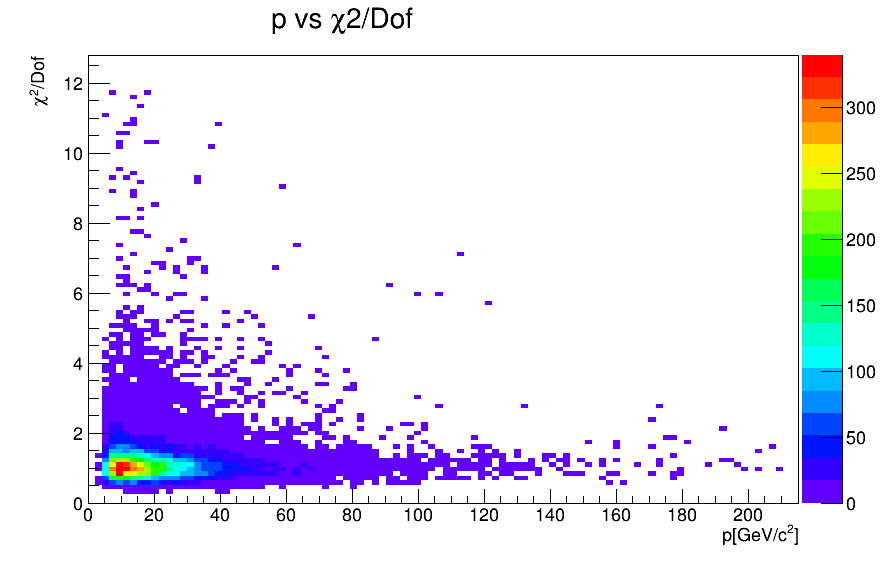
\includegraphics[width=\linewidth]{rozdzial6/JPsi_p_chi2.png}
\end{minipage}
\hspace{\fill}
\begin{minipage}[t]{0.5\textwidth}
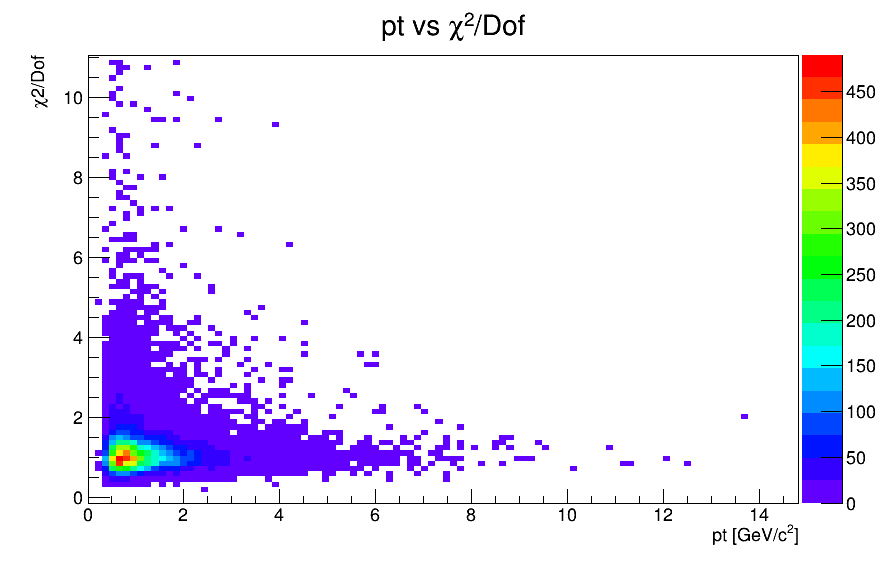
\includegraphics[width=\linewidth]{rozdzial6/JPsi_pt_chi2.png}
\end{minipage}
\caption{Korelacie pomiędzy $\chi^2_{total}$  a (góra lewo) pseudorapidity, (góra prawo) masą niezmieniczą układu pionów oraz pędami całkowitym (dół lewo) oraz poprzecznym (dół lewo). Ślady pochodzą z rozpadu $K_s$ } \label{corr_chi2JPsi}
\end{figure}

\begin{figure}[H]    
\begin{minipage}[t]{0.35\textwidth}
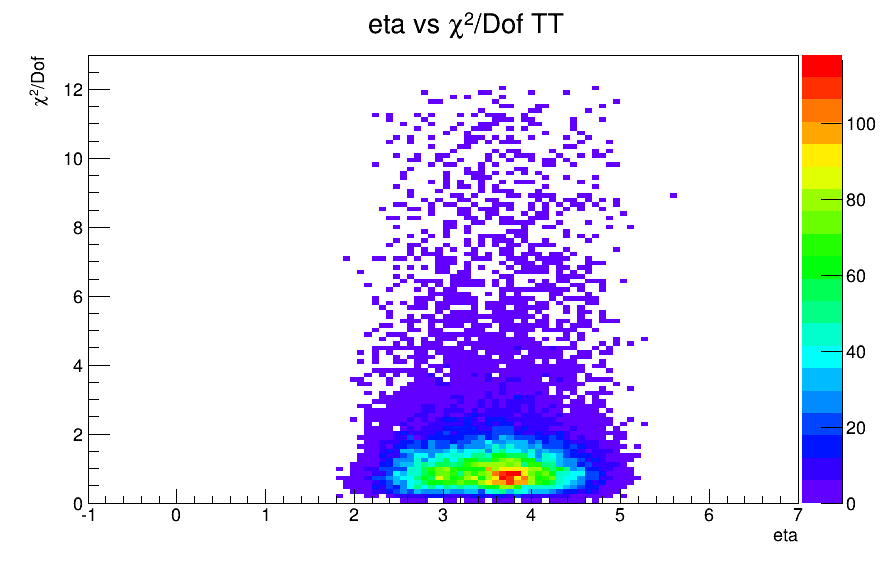
\includegraphics[width=\linewidth]{rozdzial6/JPsi_eta_chi2TT.png}
\end{minipage}
\hspace{\fill}
\begin{minipage}[t]{0.35\textwidth}
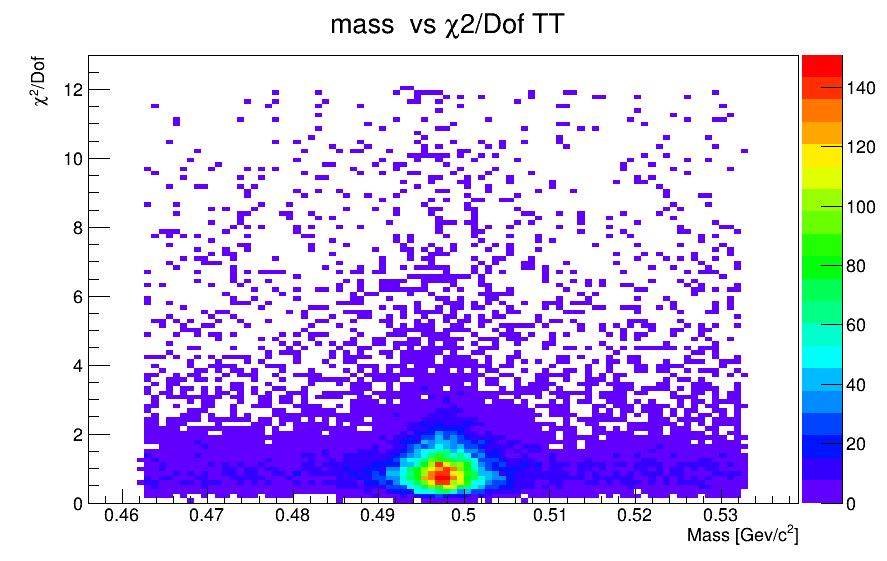
\includegraphics[width=\linewidth]{rozdzial6/JPsi_mass_chi2TT.png}
\end{minipage}

\vspace*{0.5cm} % (or whatever vertical separation you prefer)
\begin{minipage}[t]{0.35\textwidth}
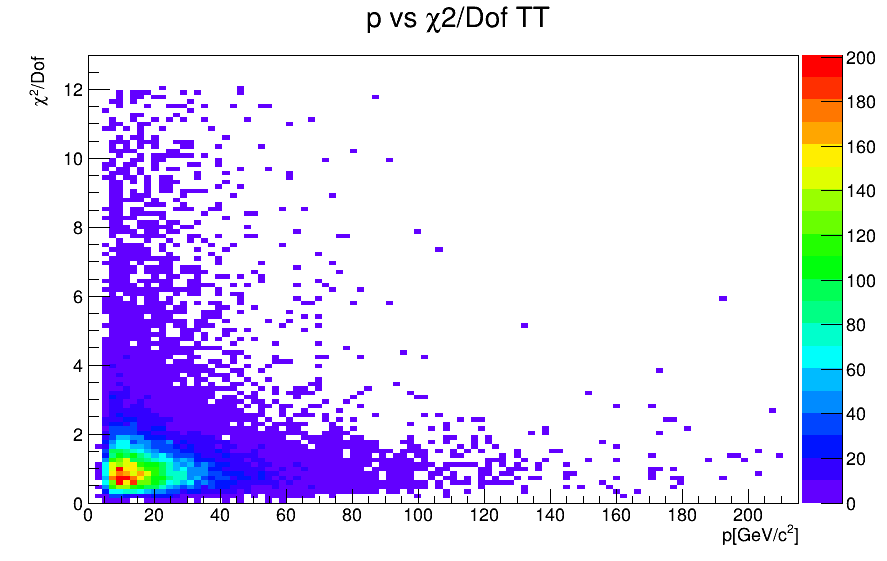
\includegraphics[width=\linewidth]{rozdzial6/JPsi_p_chi2TT.png}
\end{minipage}
\hspace{\fill}
\begin{minipage}[t]{0.35\textwidth}
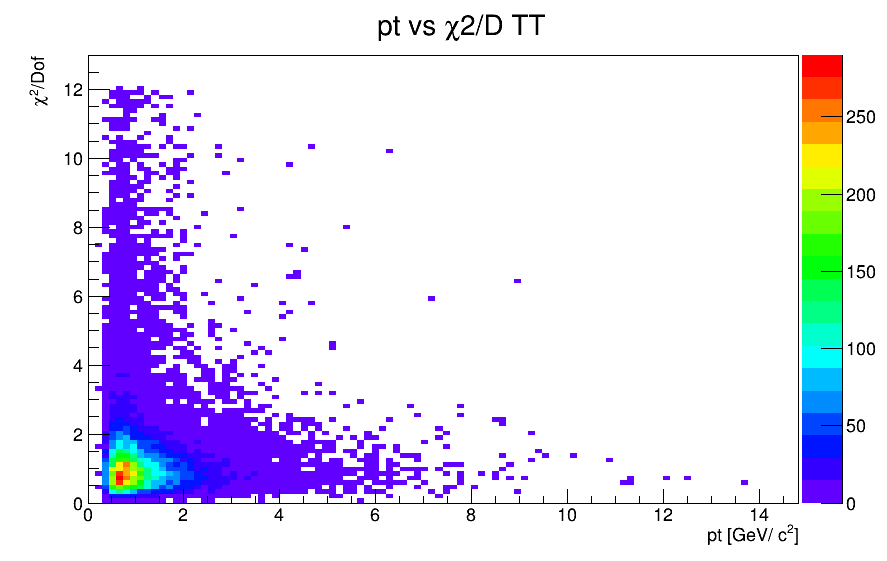
\includegraphics[width=\linewidth]{rozdzial6/JPsi_pt_chi2TT.png}
\end{minipage}
\caption{Korelacie pomiędzy $\chi^2_{TT}$ a (góra lewo) pseudorapidity, (góra prawo) masą niezmieniczą układu pionów oraz pędami całkowitym (dół lewo) oraz poprzecznym (dół lewo). Ślady pochodzą z rozpadu $K_s$. } \label{corr_chi2JPsiTT}
\end{figure} 

Analizując wyniki przedstawione na rysunkach \ref{corr_chi2JPsi} oraz \ref{corr_chi2JPsiTT} nie zaobserwowano żadnych znaczących ani widocznych korelacji pomiędzy $\chi^2$ a pseudorapidity czy masą niezmienniczą układu dwóch pionów.  Ciekawsze natomiast z punktu przeprowadzanych badań są wykresy korelacyjne zawierające informacje na temat zależności pomiędzy $\chi^2$ a pędem oraz pędem poprzecznym. Widać wyraźną zależność pomiędzy dużymi wartościami $\chi^2$ oraz małymi pędu. Równocześnie praktycznie wszystkie niefizyczne czyli zbyt małe wartości $\chi^2$ odpowiadają małym pędom. 

Ostatnim elementem, który został zrealizowany jest oparty na zbadaniu zależności jakości śladu w zależności od pozycji w detektorze TT. Widać wyraźną zależność pogorszenia jakości śladu wraz z oddalaniem się od rury akceleratora. 

 \begin{figure}[H]
 \centering
 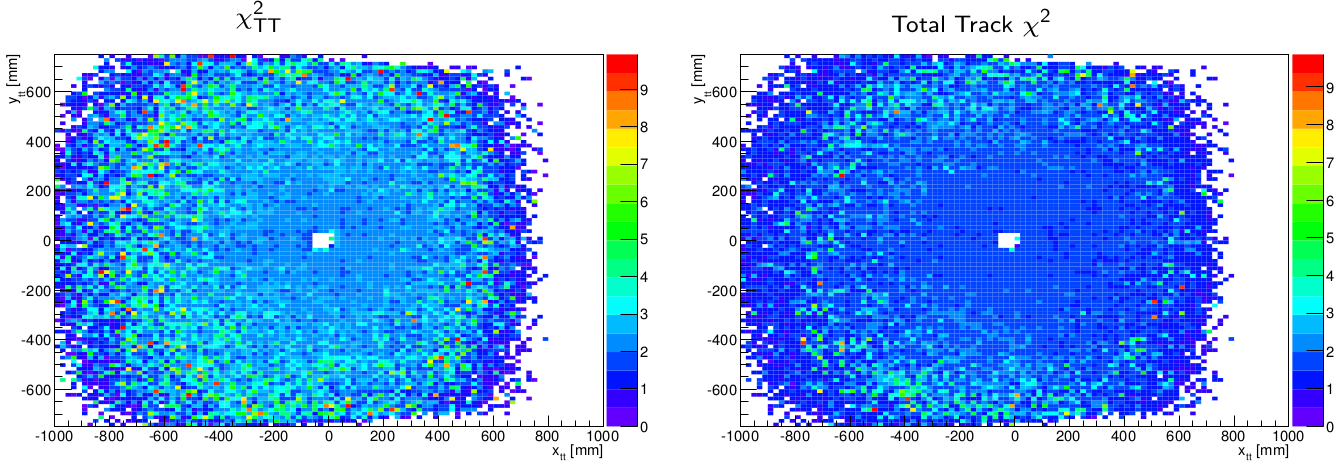
\includegraphics[scale=0.35]{rozdzial6/Chi2_vs_position_TT.png}
 % GAUDI.jpeg: 767x379 pixel, 96dpi, 20.29x10.03 cm, bb=0 0 575 284
 \caption{Zależność $\chi^2$ od pozycji śladu w detektorze TT. Po lewo znajduje się $\chi^2_{total}$, po prawo $\chi^2_{TT}$. }
 \label{rys:BJPsi}
\end{figure}

\section{Analiza oparta na danych}
Kolejnym, wykonywanym równolegle krokiem była analiza oparta na danych zabranych przez detektor. Wybrane przypadki pochodzą z linii strippingowej o nazwie \\ \textbf{BetaSBd2JpsiKsDetachedLine}. Użyto cięć typu \textbf{Loose} w ten sposób chciano zwiększyć badaną statystykę. Natomiast inne, bardziej restrykcyjne cięcia zostały zastosowane podczas analizy. Jednakże warto zwrócić uwagę na fakt iż nawet te mniej restrykcyjne cięcia stosują ograniczenie $\chi^2_{total}<3$. 

\subsection{Rozkłady $\chi^2$ bazujące na danych}
Podobnie jak dla danych MC wykonano rozkłady $\chi^2$. Również w tym przypadku prawdziwa jest zależność \ref{chiTotal}. 

\begin{figure}[H]    
\begin{minipage}[t]{0.55\textwidth}
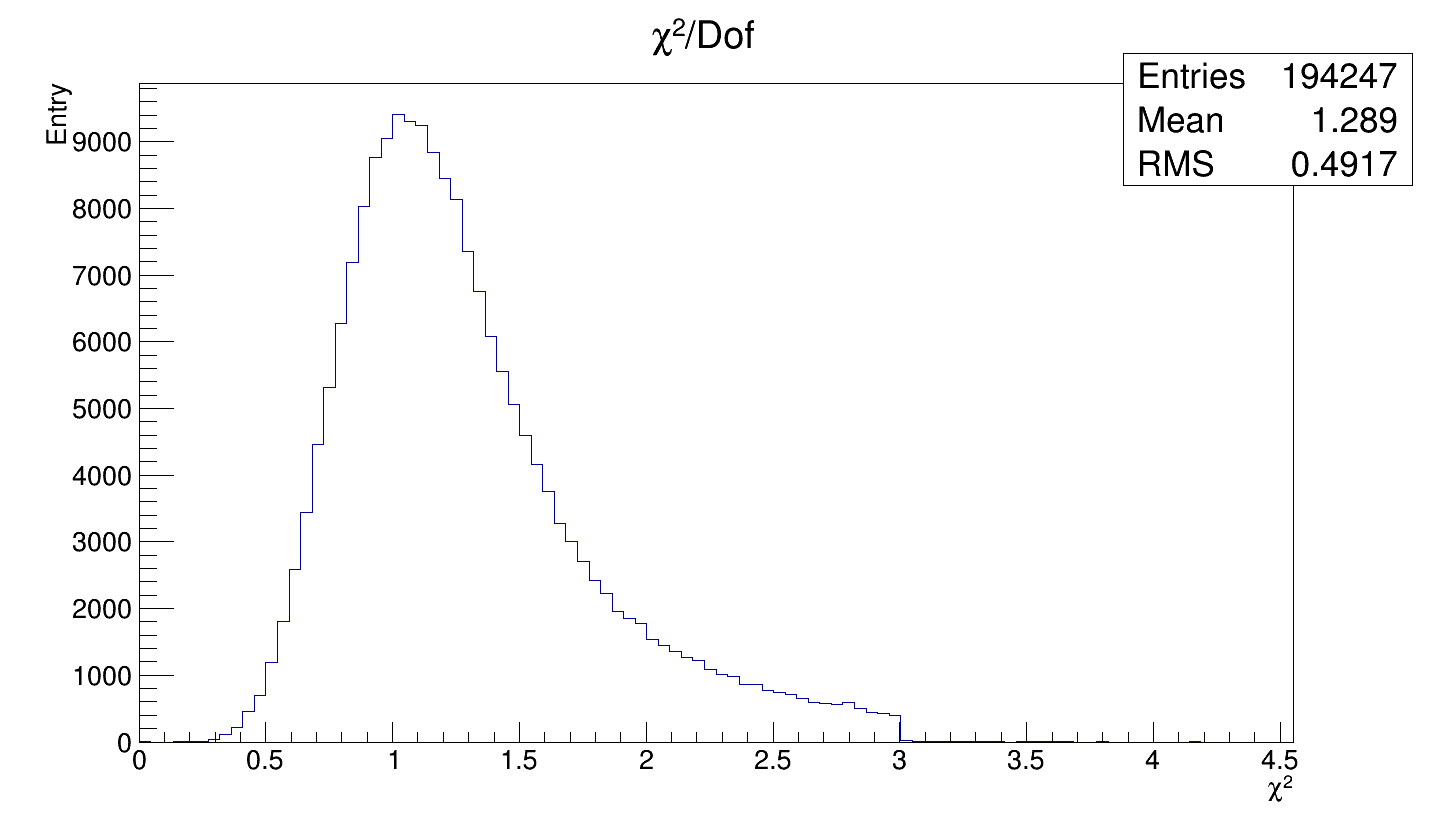
\includegraphics[width=\linewidth]{rozdzial6/JPsi_chi2_data.png}
\end{minipage}
\hspace{\fill}
\begin{minipage}[t]{0.55\textwidth}
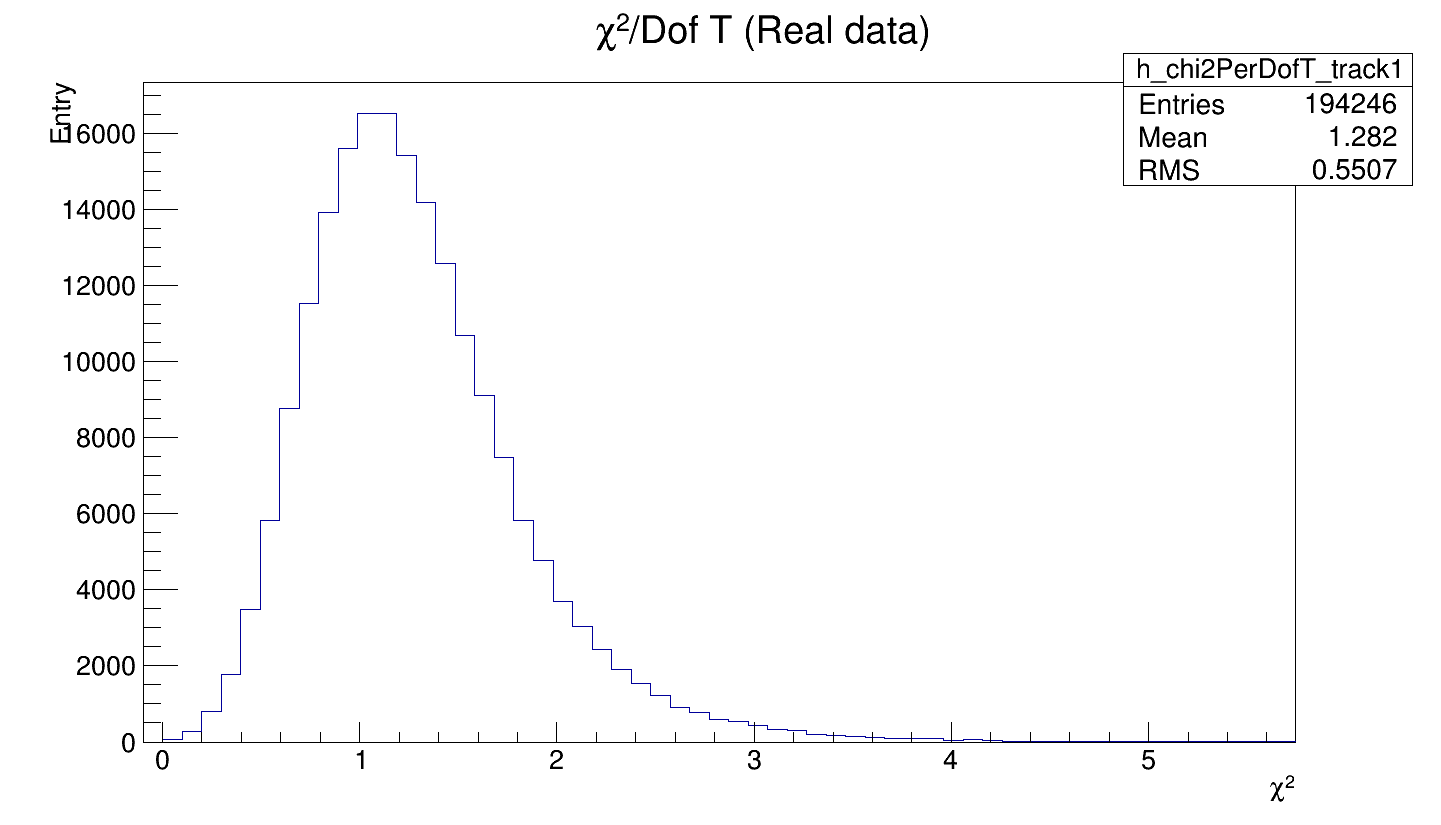
\includegraphics[width=\linewidth]{rozdzial6/JPsi_chi2T_data.png}
\end{minipage}

\vspace*{0.5cm} % (or whatever vertical separation you prefer)
\begin{minipage}[t]{0.55\textwidth}
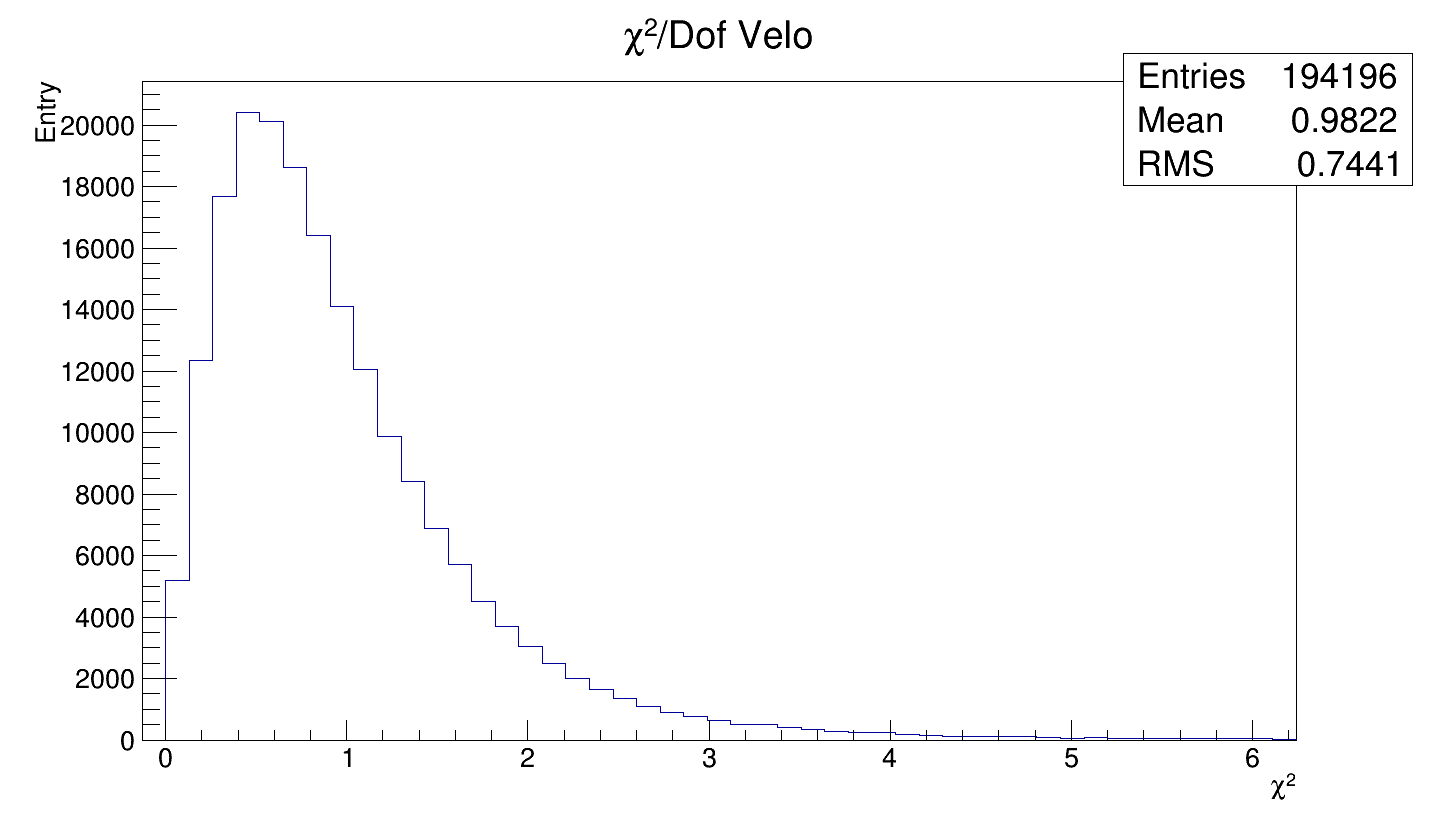
\includegraphics[width=\linewidth]{rozdzial6/JPsi_chi2Velo_data.png}
\end{minipage}
\hspace{\fill}
\begin{minipage}[t]{0.55\textwidth}
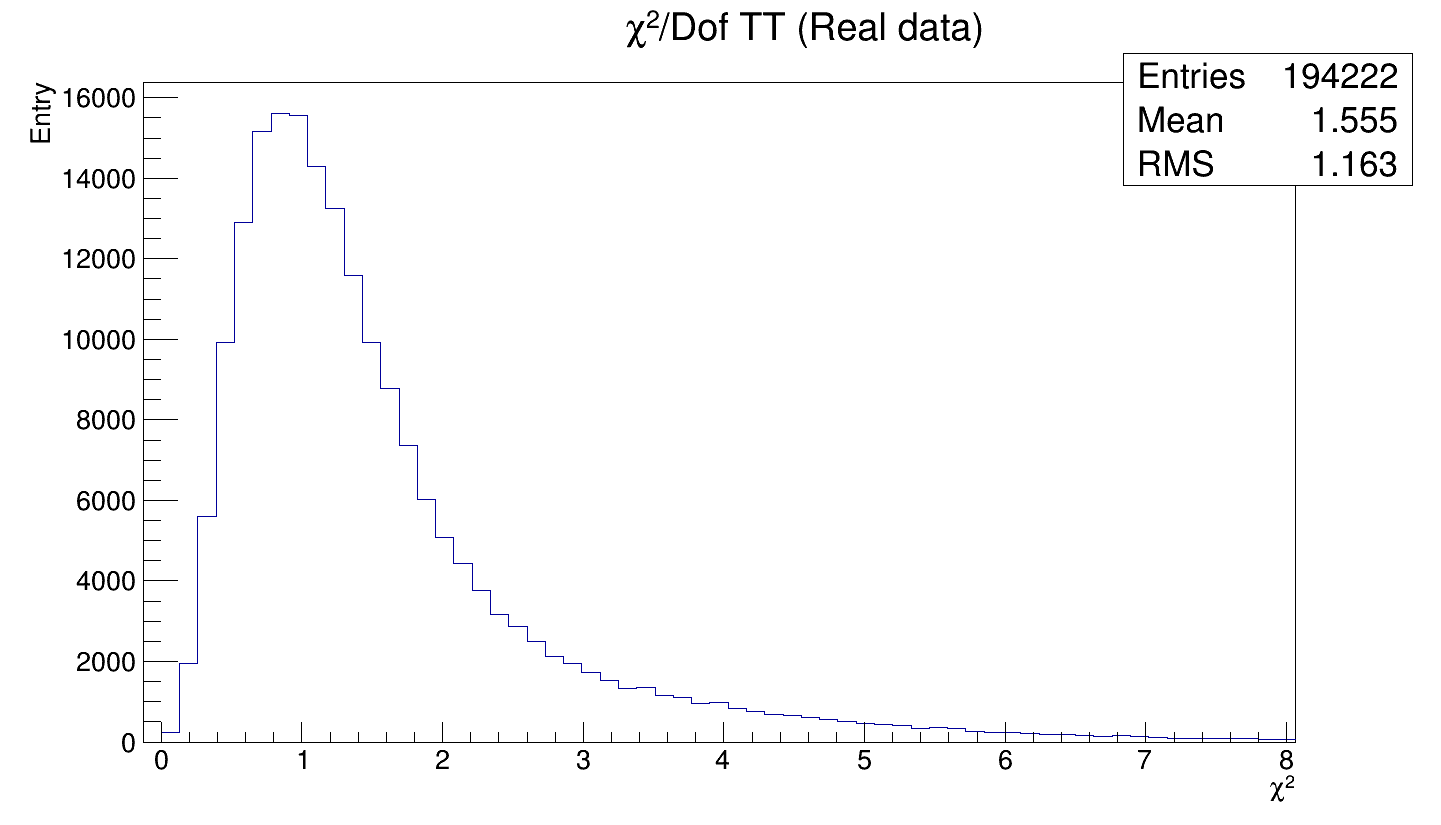
\includegraphics[width=\linewidth]{rozdzial6/JPsi_chi2TT_data.png}
\end{minipage}
\caption{Rozkłady $\chi^2$ wyliczone dla śladów zrekonstruowanych w wyniku oddziaływania produktów rozpadu mezonu $J/\Psi$. Na rysunku (góra lewo) przedstawiono całkowity $\chi^2$, na (góra prawo) rozkład dla części T, natomiast na dole rozkłady dla Velo (lewo) oraz TT (prawo). Rozkłady wykonano bazując na danych rzeczywistych, zebranych przez układ detekcyjny LHCb.} \label{chi2JPsi_data}
\end{figure}  

\begin{figure}[h]    
\begin{minipage}[t]{0.45\textwidth}
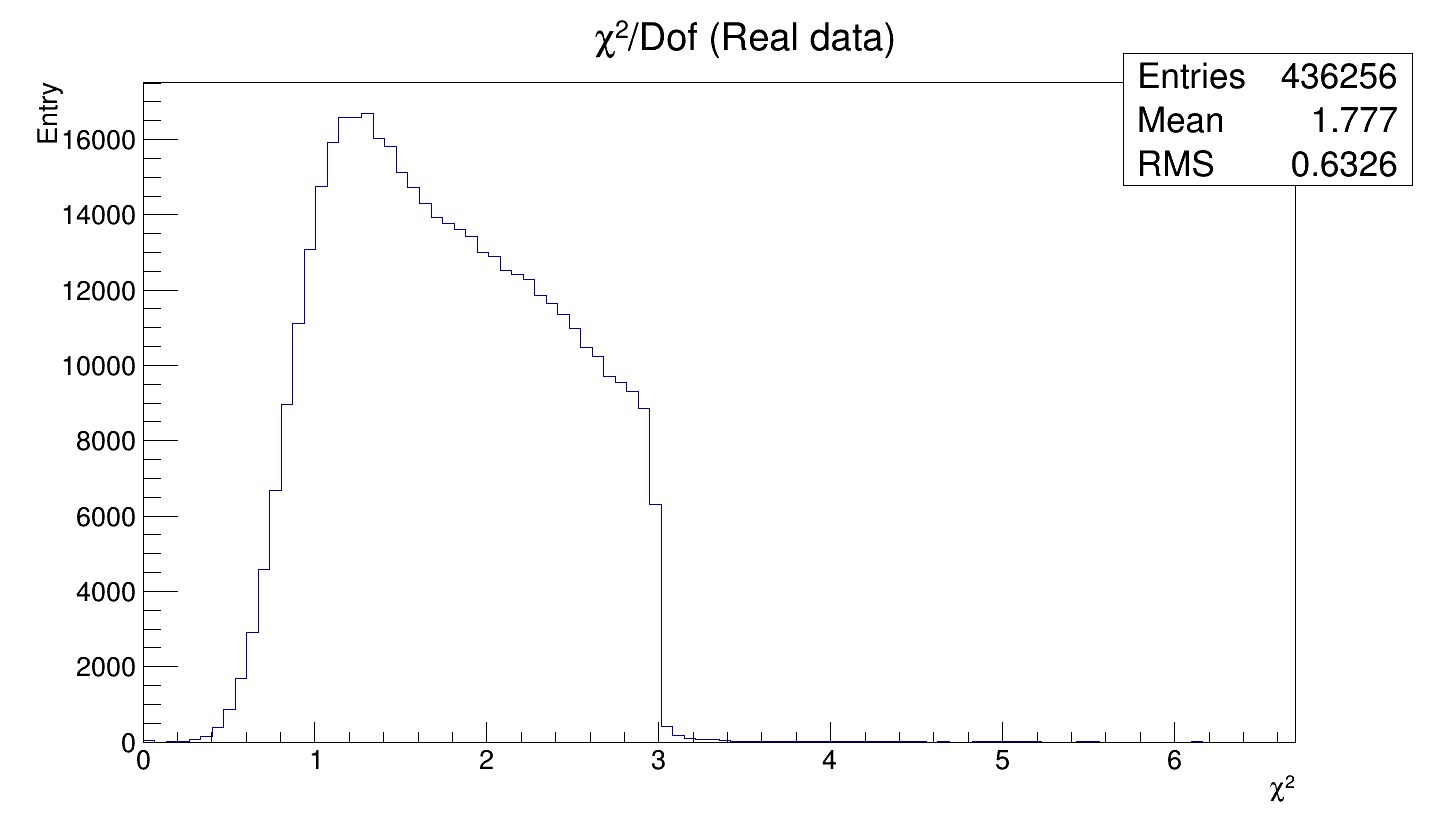
\includegraphics[width=\linewidth]{rozdzial6/KsLL_chi2_data.png}
\end{minipage}
\hspace{\fill}
\begin{minipage}[t]{0.45\textwidth}
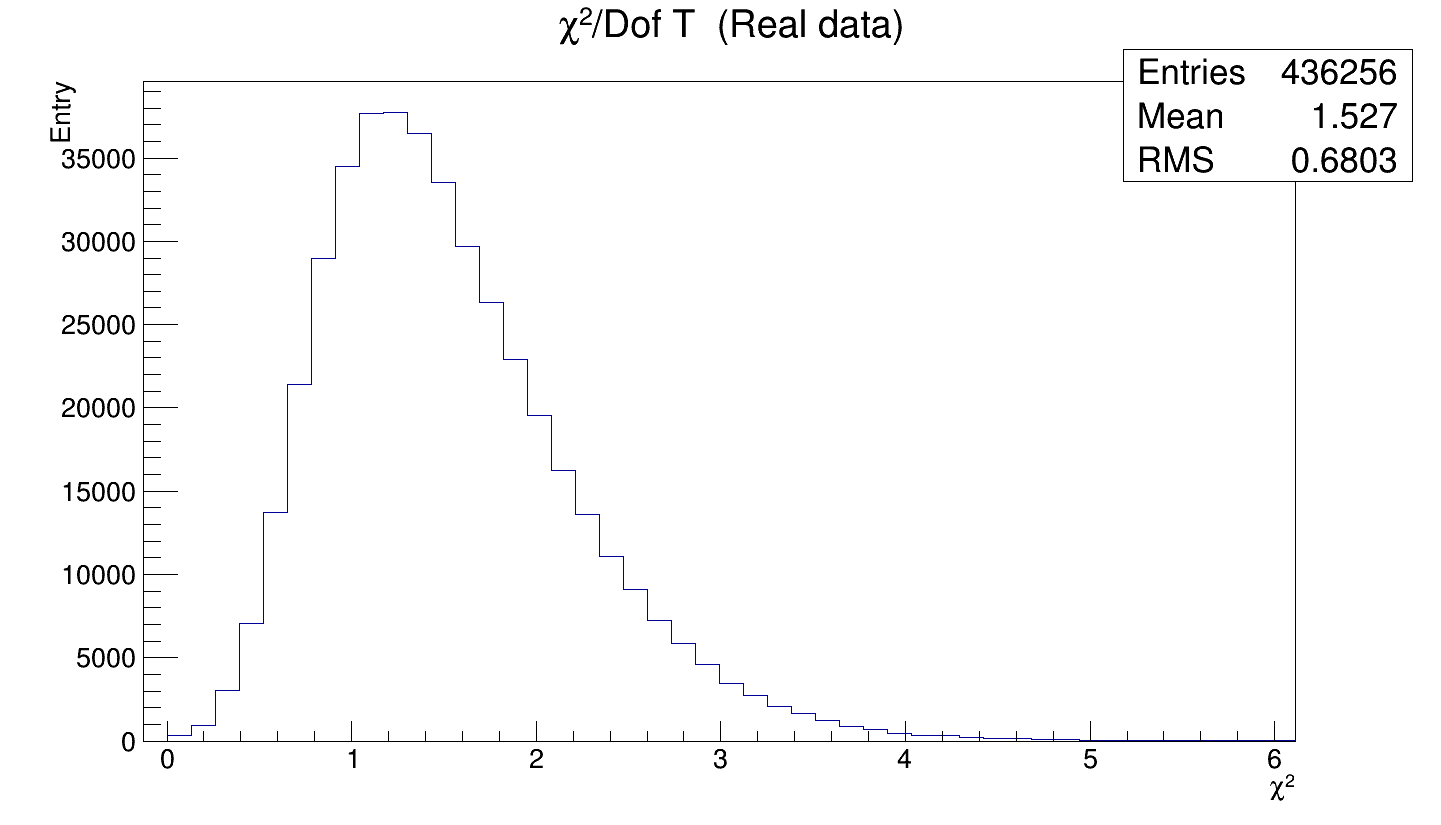
\includegraphics[width=\linewidth]{rozdzial6/KsLL_chi2T_data.png}
\end{minipage}

\vspace*{0.5cm} % (or whatever vertical separation you prefer)
\begin{minipage}[t]{0.45\textwidth}
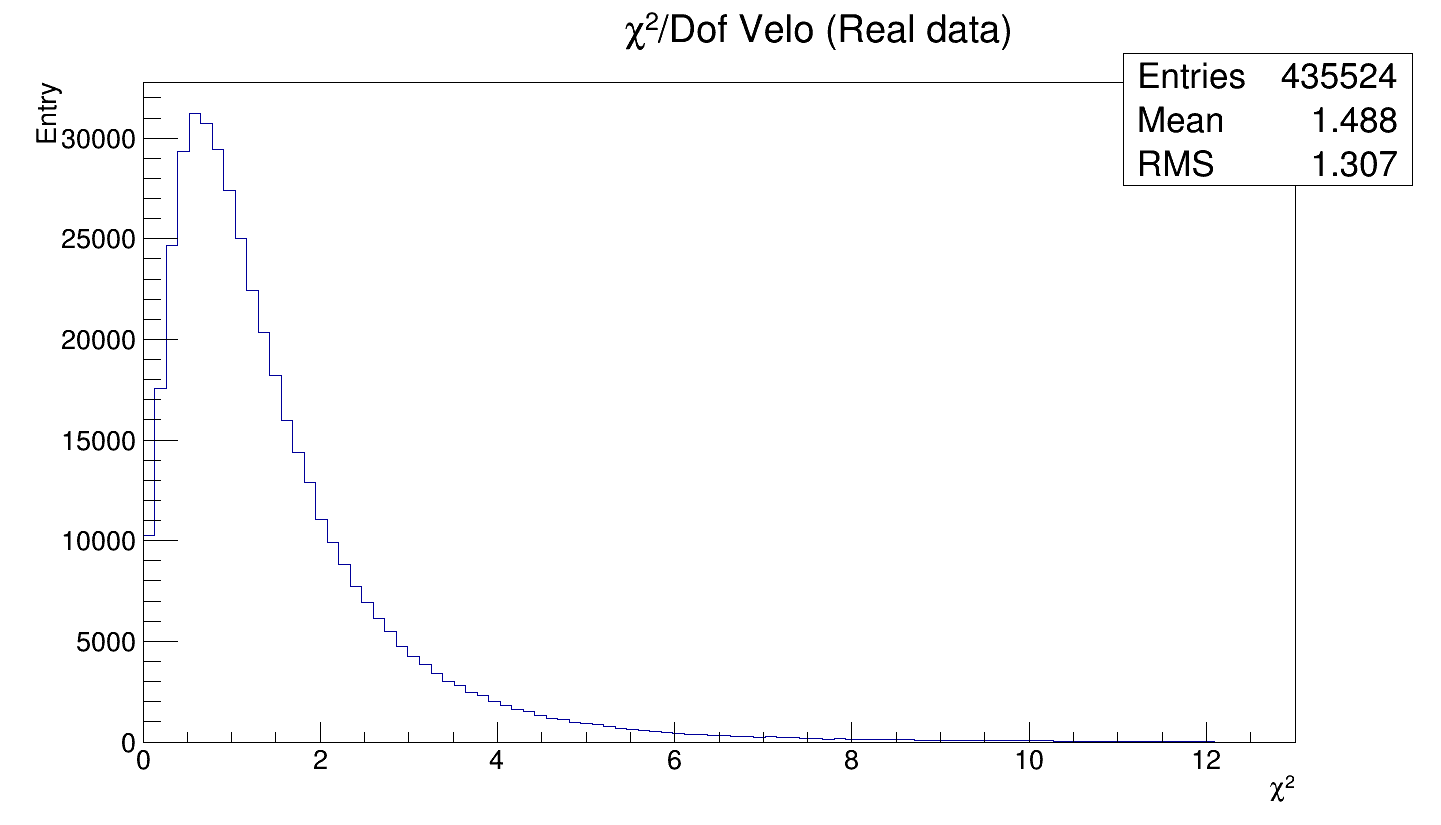
\includegraphics[width=\linewidth]{rozdzial6/KsLL_chi2Velo_data.png}
\end{minipage}
\hspace{\fill}
\begin{minipage}[t]{0.5\textwidth}
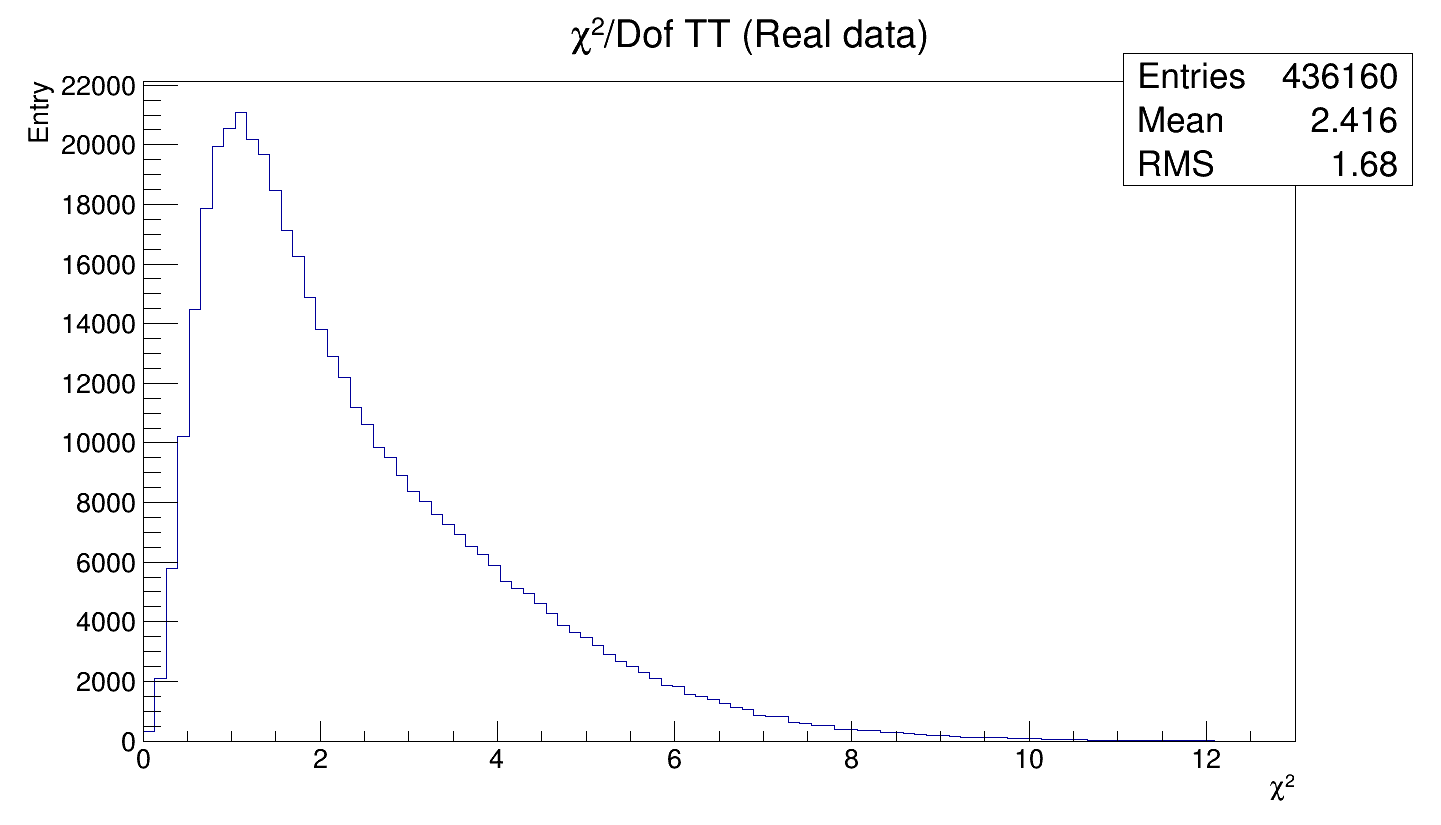
\includegraphics[width=\linewidth]{rozdzial6/KsLL_chi2TT_data.png}
\end{minipage}
\caption{Rozkłady $\chi^2$ wyliczone dla śladów \textbf{długich} zrekonstruowanych w wyniku oddziaływania produktów rozpadu mezonu $Ks$. Na rysunku (góra lewo) przedstawiono całkowity $\chi^2$, na (góra prawo) rozkład dla części T, natomiast na dole rozkłady dla Velo (lewo) oraz TT (prawo). Rozkłady wykonano bazując na danych rzeczywistych, zebranych przez układ detekcyjny LHCb.} \label{chi2KsLL_data}
\end{figure}

Najciekawszym, zaobserwowanym  zjawiskiem jest występowanie długiego ogona w rozkładzie $\chi^2_{TT}$, na rysunku \ref{chi2KsLL_data}. Ogon ten znacząco wpływa na wartość $\chi^2_{total}$. Obserwacja ta jest dość istotna, zważając na poczynione cięcia. Wpływ niedostatecznej wydajności rekonstrukcji śladów przez detektor TT może powodować niepotrzebną eliminację  przypadków. Wynika to z cięcia na $\chi^2_{total}$.

\subsection{Ekstrakcja sygnału od szumu}
Ważnym elementem podczas pracy z danymi zebranymi w trakcie pracy detektora jest odseparowanie rzeczywistego sygnału od szumu. W tym celu wykorzystano technikę zwaną \textbf{sPlot}. Dokładny opis wraz z pełnym matematycznym wyprowadzeniem tej techniki można znaleźć w referencji \cite{sPlot}. Z technicznego punktu widzenia zadanie to wymagało wykorzystania pakietu Roofit. 

Jako model, który został dopasowywany do danych wybrano sumę dwóch rozkładów Gaussa natomiast za model tła przyjęto rozkład eksponencjalny. Na rysunku \ref{massJPsi} zamieszczono zrekonstruowany rozkład masy mezonu $J / \Psi$  wraz z dopasowanym wyżej opisanym modelem. Korzystając z tych wyników udało się wyekstrahować sygnał od szumu. Następnie narysowano najbardziej istotne rozkłady $\chi^2_{total}$ oraz $\chi^2_{TT}$. Wyniki zamieszczono na rysunku \ref{chi2sPlot}. Zauważono brak widocznych korelacji pomiędzy szumem a jakością dopasowania śladów. Podobne wyniki daje analiza oparta na śladach pochodzących z rozpadu $K_s$, niezależnie czy badano ślady długie czy typu downstream. 

\begin{figure}[H]    
\begin{minipage}[t]{0.6\textwidth}
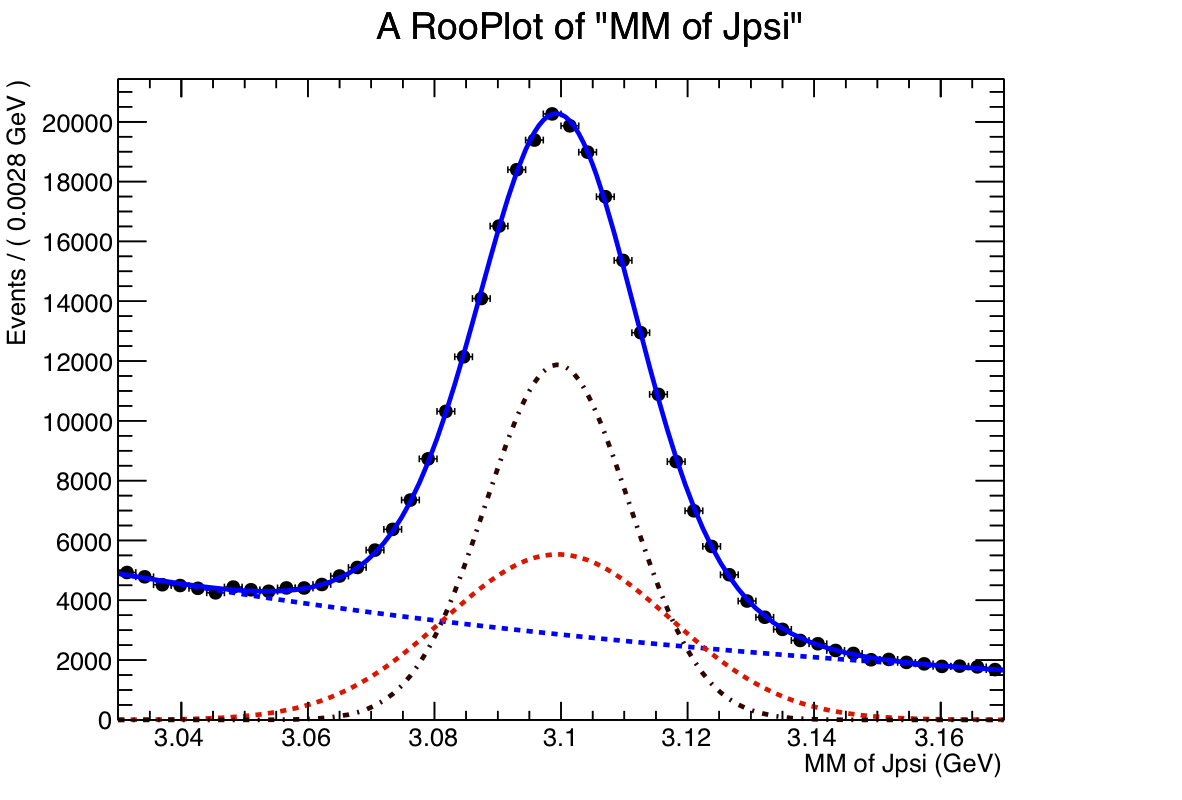
\includegraphics[width=\linewidth]{rozdzial6/jpsi_mm_sPlot_RDfit.png}
\end{minipage}
\hspace{\fill}
\begin{minipage}[t]{0.5\textwidth}
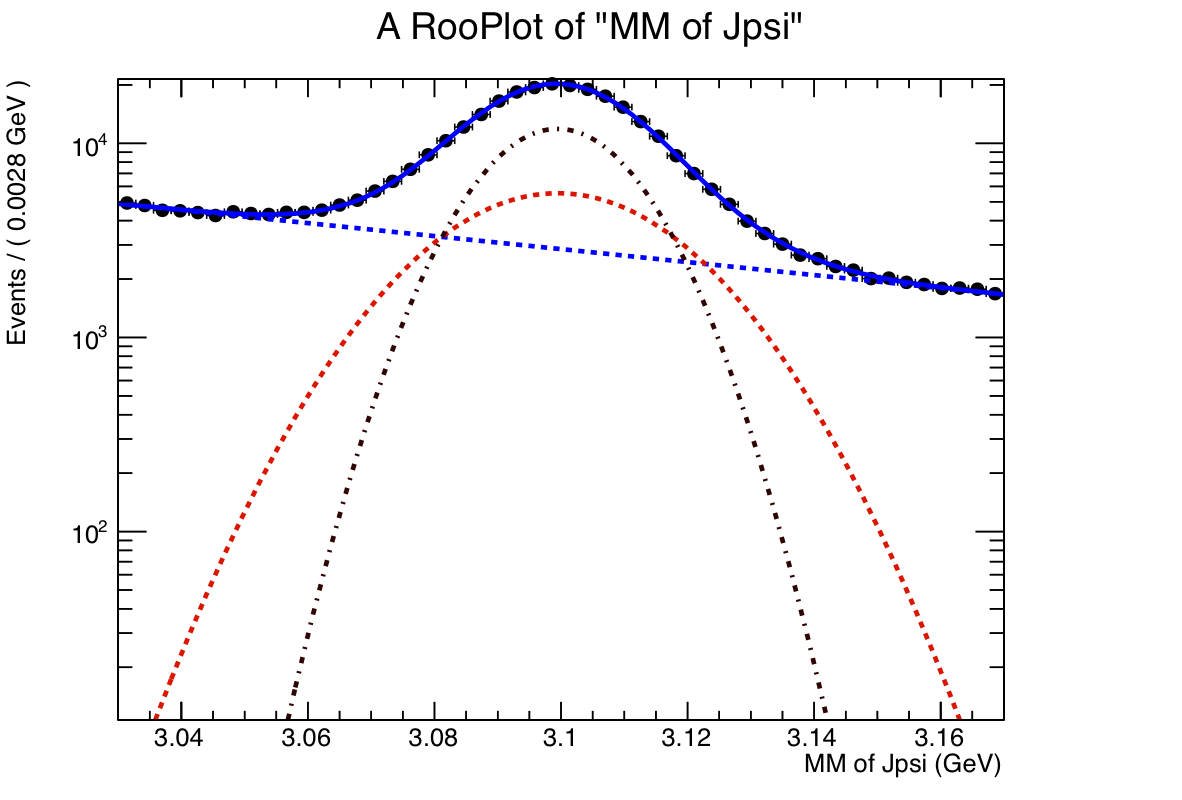
\includegraphics[width=\linewidth]{rozdzial6/jpsi_mm_sPlot_RDfit_logy.png}
\end{minipage}
\caption{Rozkład masy niezmienniczej układu mionów wraz z dopasowanym modelem sumy dwóch rozkładów normalnych ( kropkowane czerwona i czarna linia) oraz eksponencjalnym tłem (niebieska kropkowana linia). Wykres po prawej posiada os Y w skali logarytmicznej.} \label{massJPsi}
\end{figure} 


\begin{figure}[H]    
\begin{minipage}[t]{0.6\textwidth}
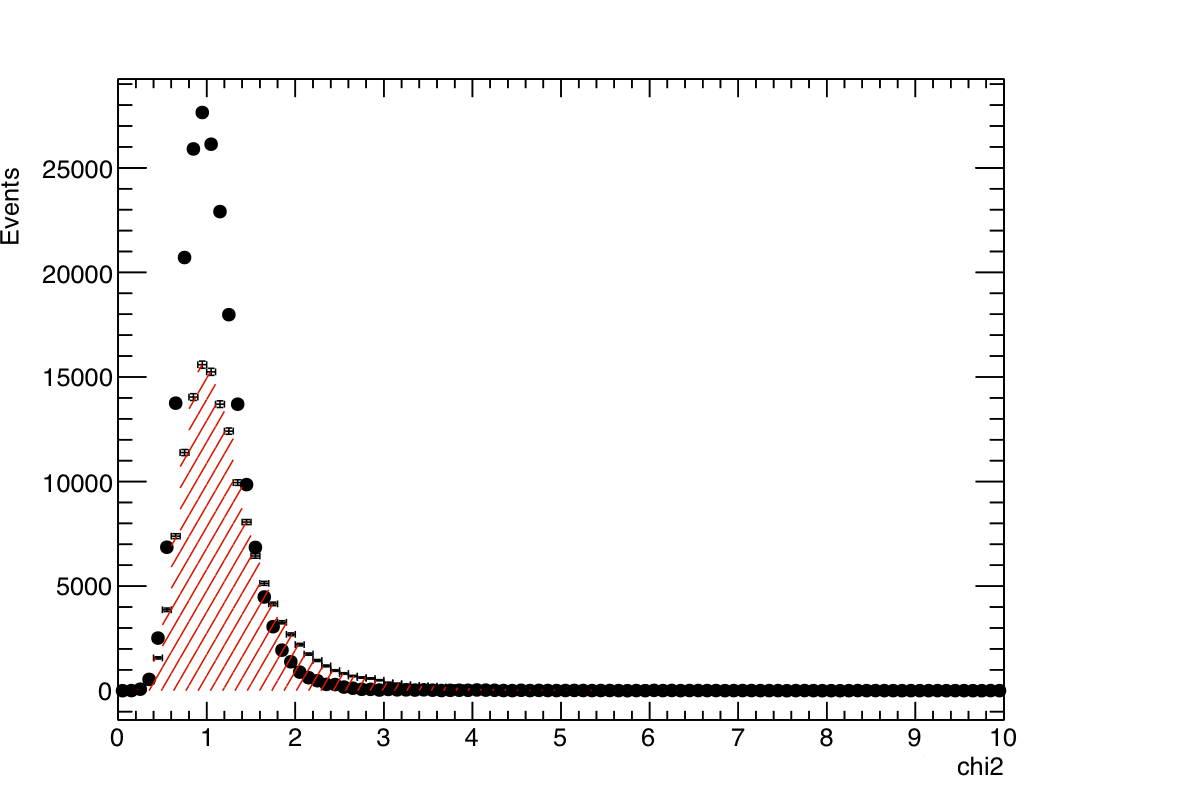
\includegraphics[width=\linewidth]{rozdzial6/jpsi_chi2_sPlot.png}
\end{minipage}
\hspace{\fill}
\begin{minipage}[t]{0.5\textwidth}
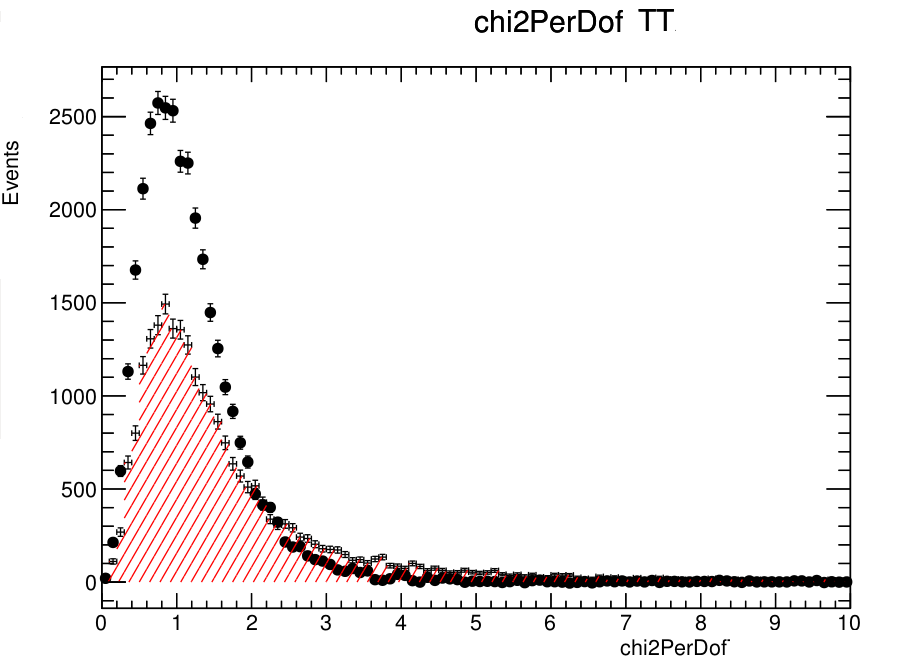
\includegraphics[width=\linewidth]{rozdzial6/jpsi_chi2TT_sPlot.png}
\end{minipage}
\caption{Rozkład $\chi^2$ dla wyselekcjonowanego szumu (oznaczony na czerwono) oraz dla sygnału. Po lewej zamieszczono wykres dla $\chi^2_{total}$ natomiast po prawej $\chi_{TT}^2$} \label{chi2sPlot}
\end{figure} 

\subsection{Zależności korelacyjne}
Ostatnim elementem, który został wykonany w tym stadium analizy jest przedstawienie, podobnie jak w przypadku danych Monte Carlo zależności korelacyjnych pomiędzy $\chi^2$ a innymi parametrami takimi jak pęd całkowity i poprzeczny, masę oraz pseudorapidity. W niniejszej  pracy zaprezentowano wyniki tylko dla rozpadu $J / \Psi$. Korelacje te przedstawiono na rysunkach \ref{corr_chi2JPsi_data} oraz \ref{corr_chi2JPsiTT_data}. Jakościowo rysunki te nie odróżniają się od tych, otrzymanych dla danych Monte Carlo. 

\begin{figure}[H]    
\begin{minipage}[t]{0.5\textwidth}
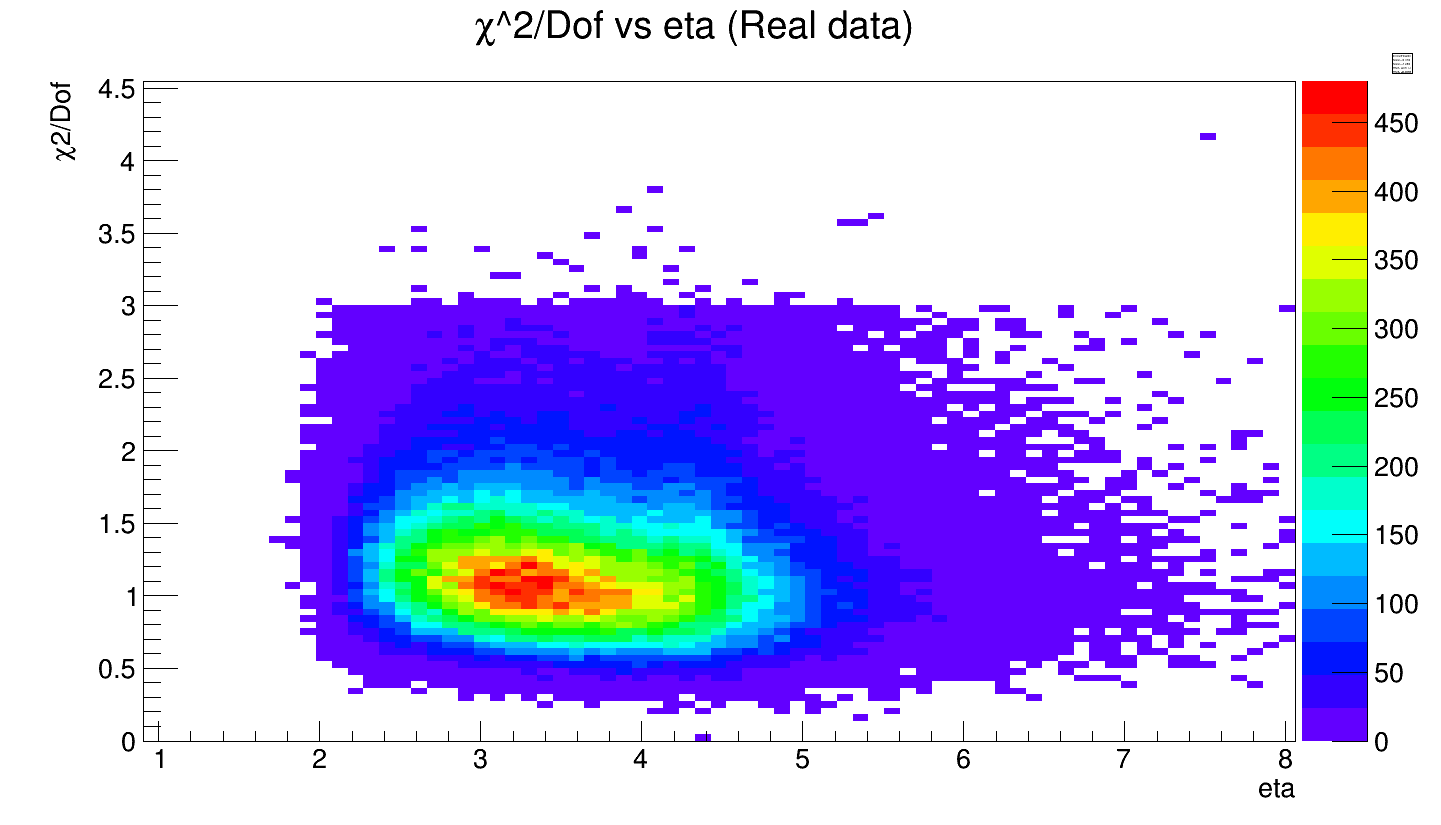
\includegraphics[width=\linewidth]{rozdzial6/JPsi_eta_chi2_data.png}
\end{minipage}
\hspace{\fill}
\begin{minipage}[t]{0.5\textwidth}
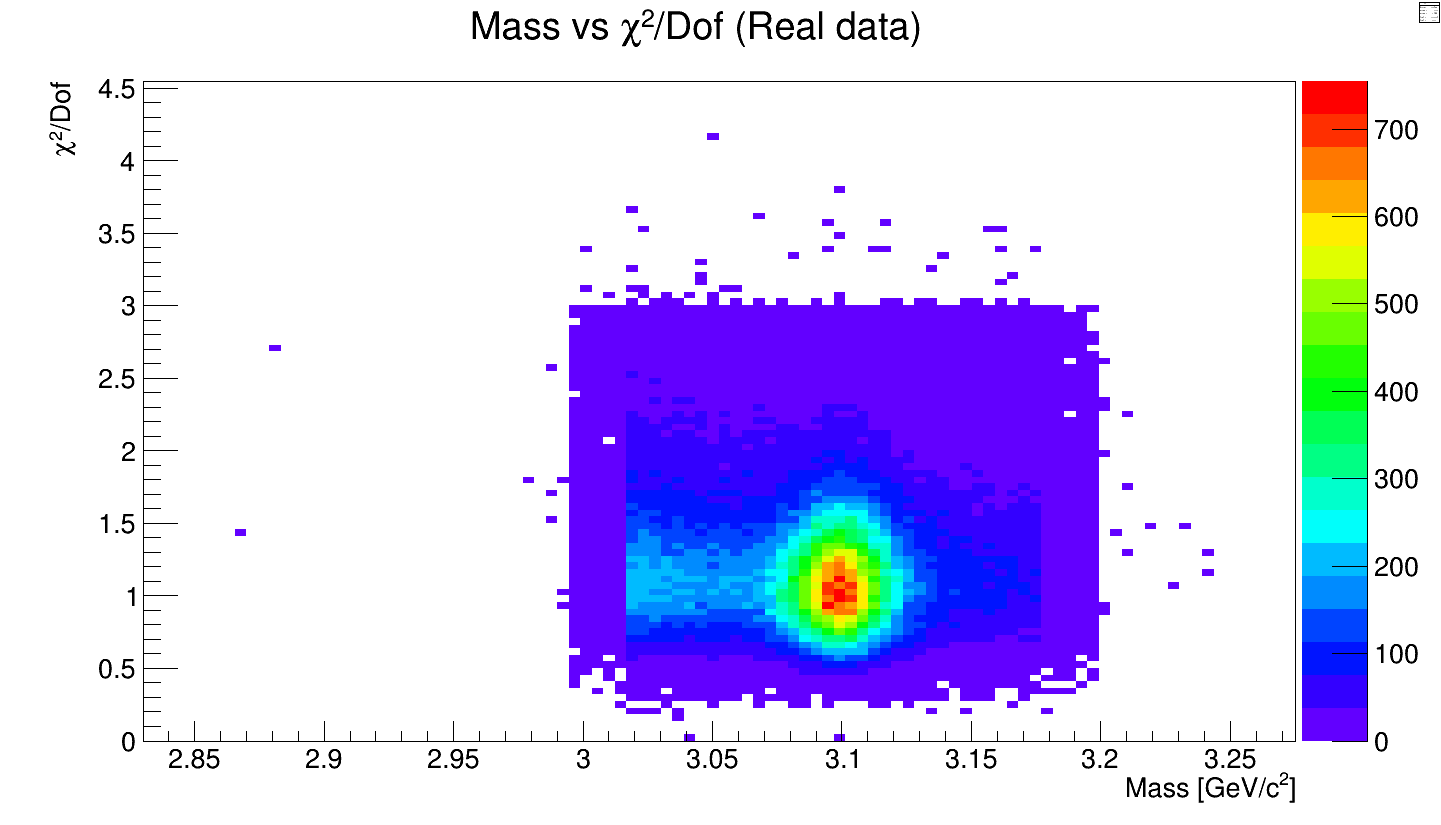
\includegraphics[width=\linewidth]{rozdzial6/JPsi_mass_chi2_data.png}
\end{minipage}

\vspace*{0.5cm} % (or whatever vertical separation you prefer)
\begin{minipage}[t]{0.5\textwidth}
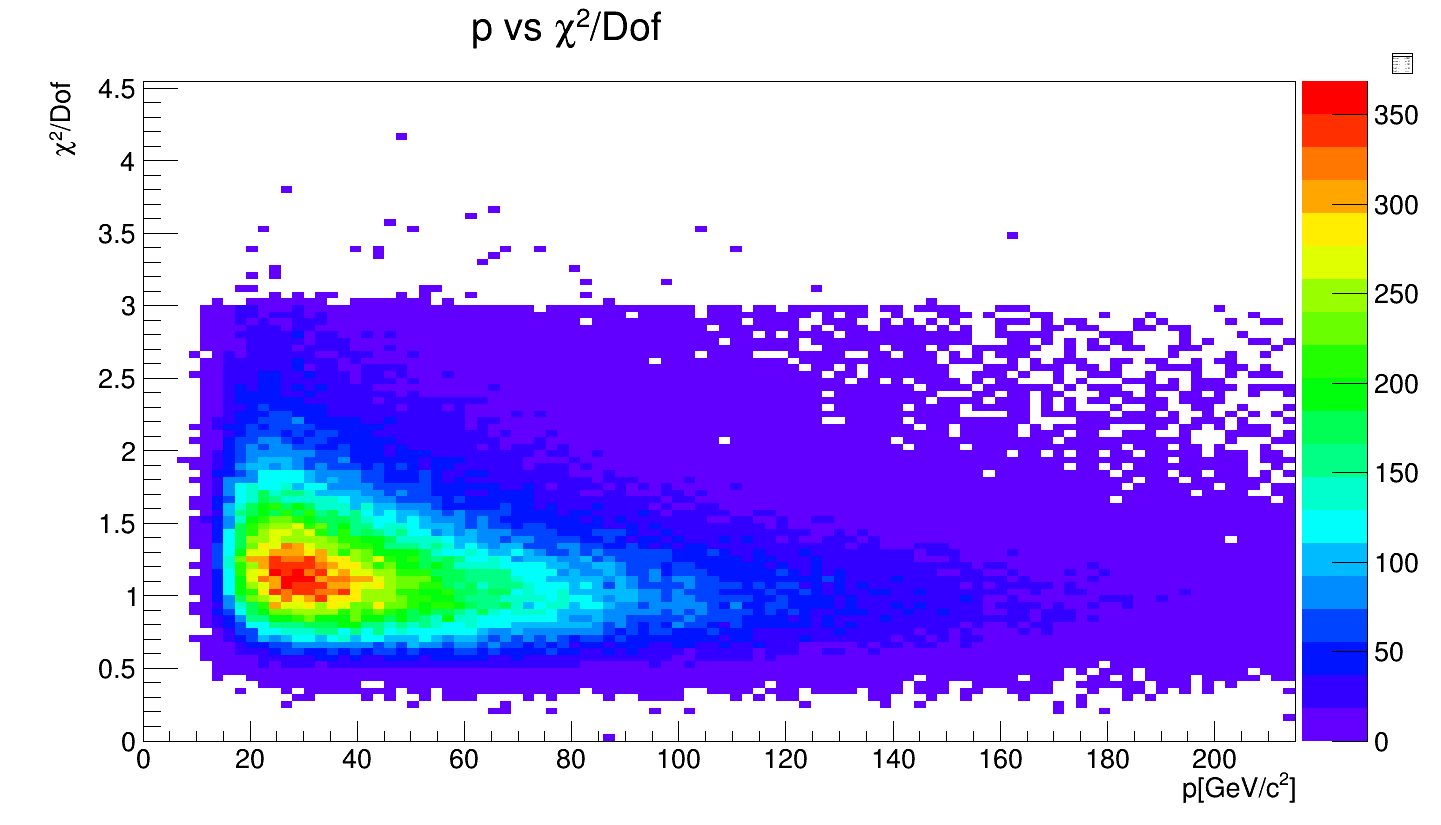
\includegraphics[width=\linewidth]{rozdzial6/JPsi_p_chi2_data.png}
\end{minipage}
\hspace{\fill}
\begin{minipage}[t]{0.5\textwidth}
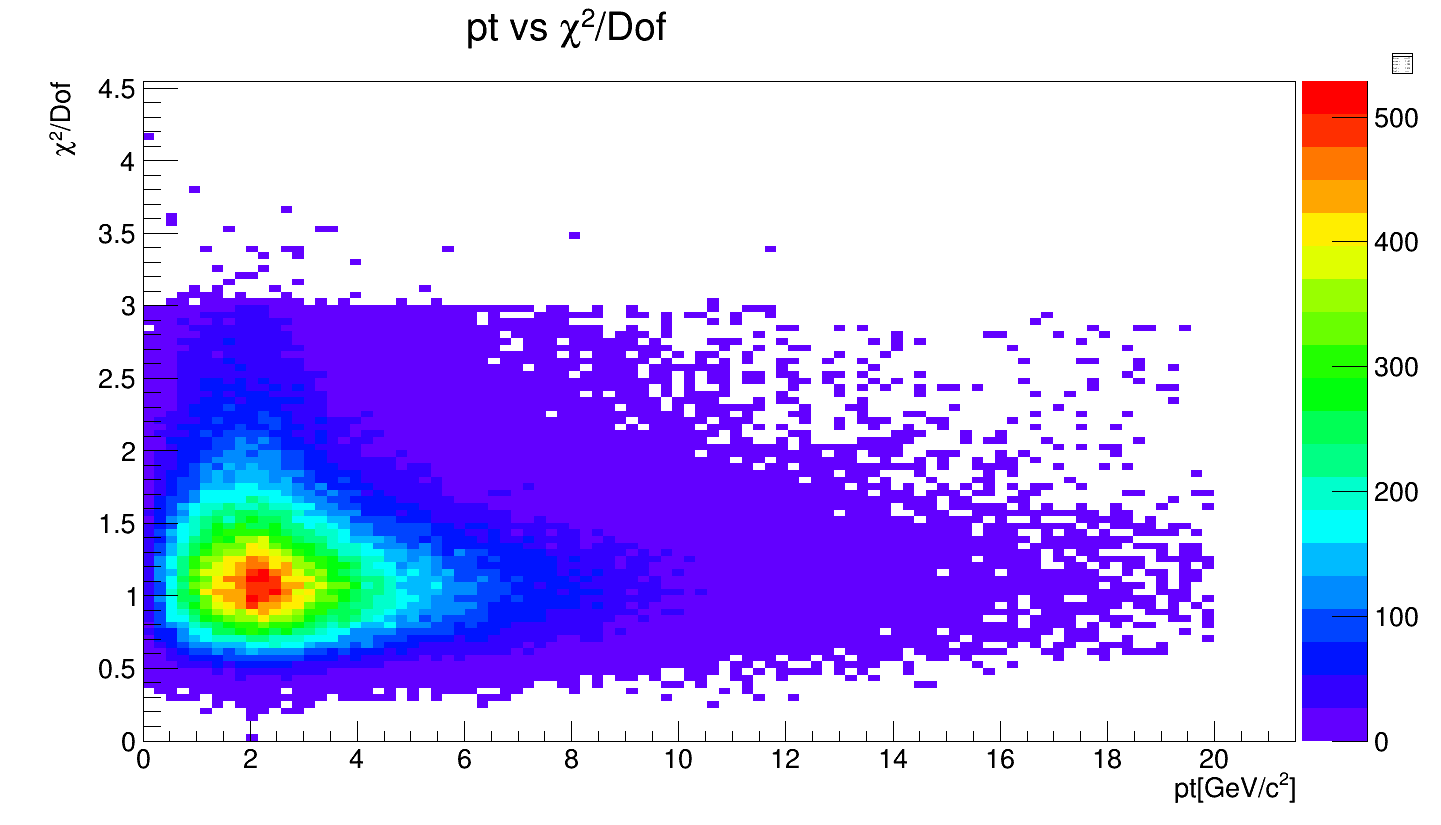
\includegraphics[width=\linewidth]{rozdzial6/JPsi_pt_chi2_data.png}
\end{minipage}
\caption{Korelacie pomiędzy $\chi^2_{total}$  a (góra lewo) pseudorapidity, (góra prawo) masą niezmieniczą układu pionów oraz pędami całkowitym (dół lewo) oraz poprzecznym (dół lewo). Ślady pochodzą z rozpadu $J / \Psi$. Wykresy wykonano bazując na danych rzeczywistych, zebranych przez układ detekcyjny LHCb.} \label{corr_chi2JPsi_data}
\end{figure}

\begin{figure}[H]    
\begin{minipage}[t]{0.5\textwidth}
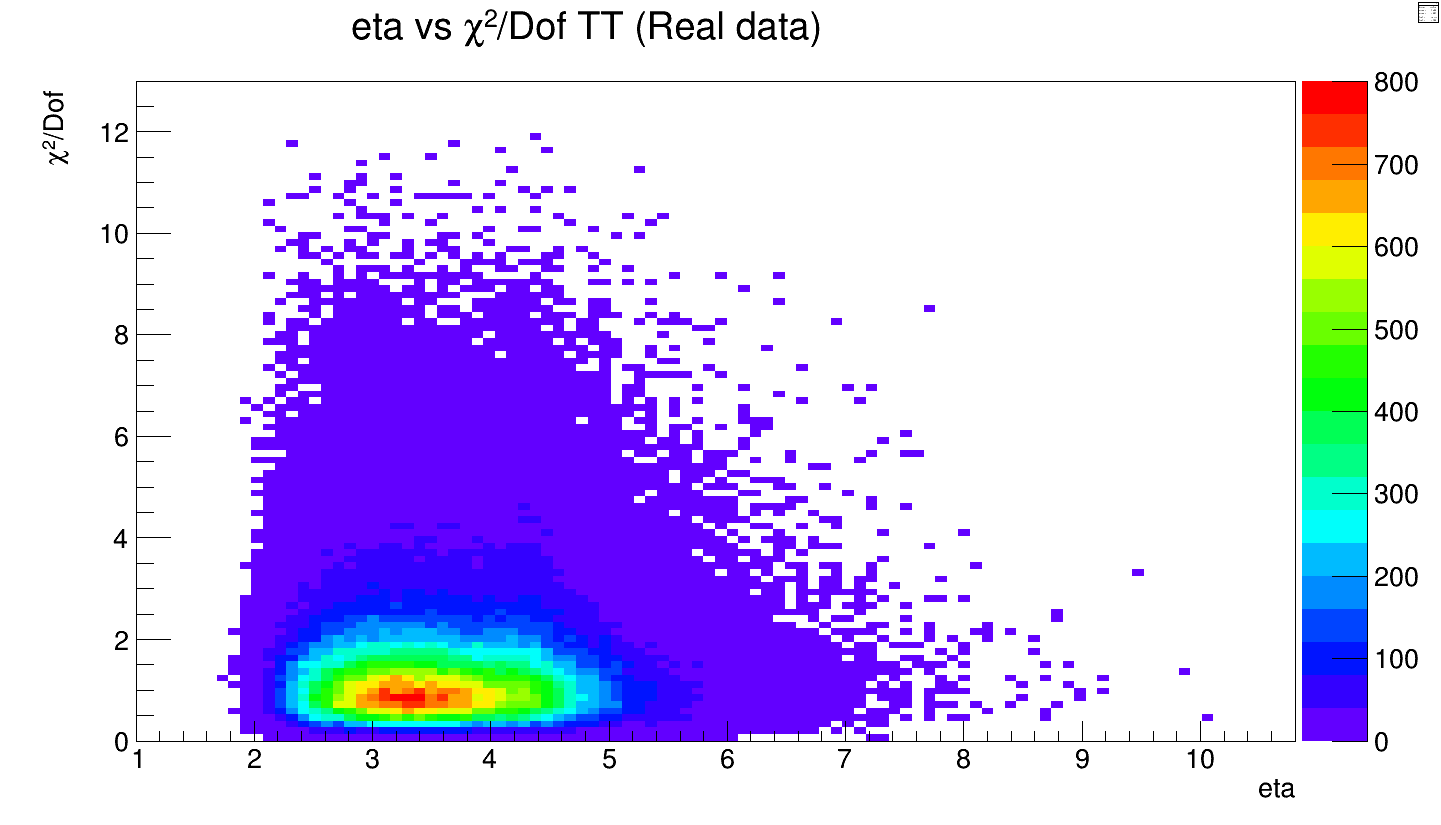
\includegraphics[width=\linewidth]{rozdzial6/JPsi_eta_chi2TT_data.png}
\end{minipage}
\hspace{\fill}
\begin{minipage}[t]{0.5\textwidth}
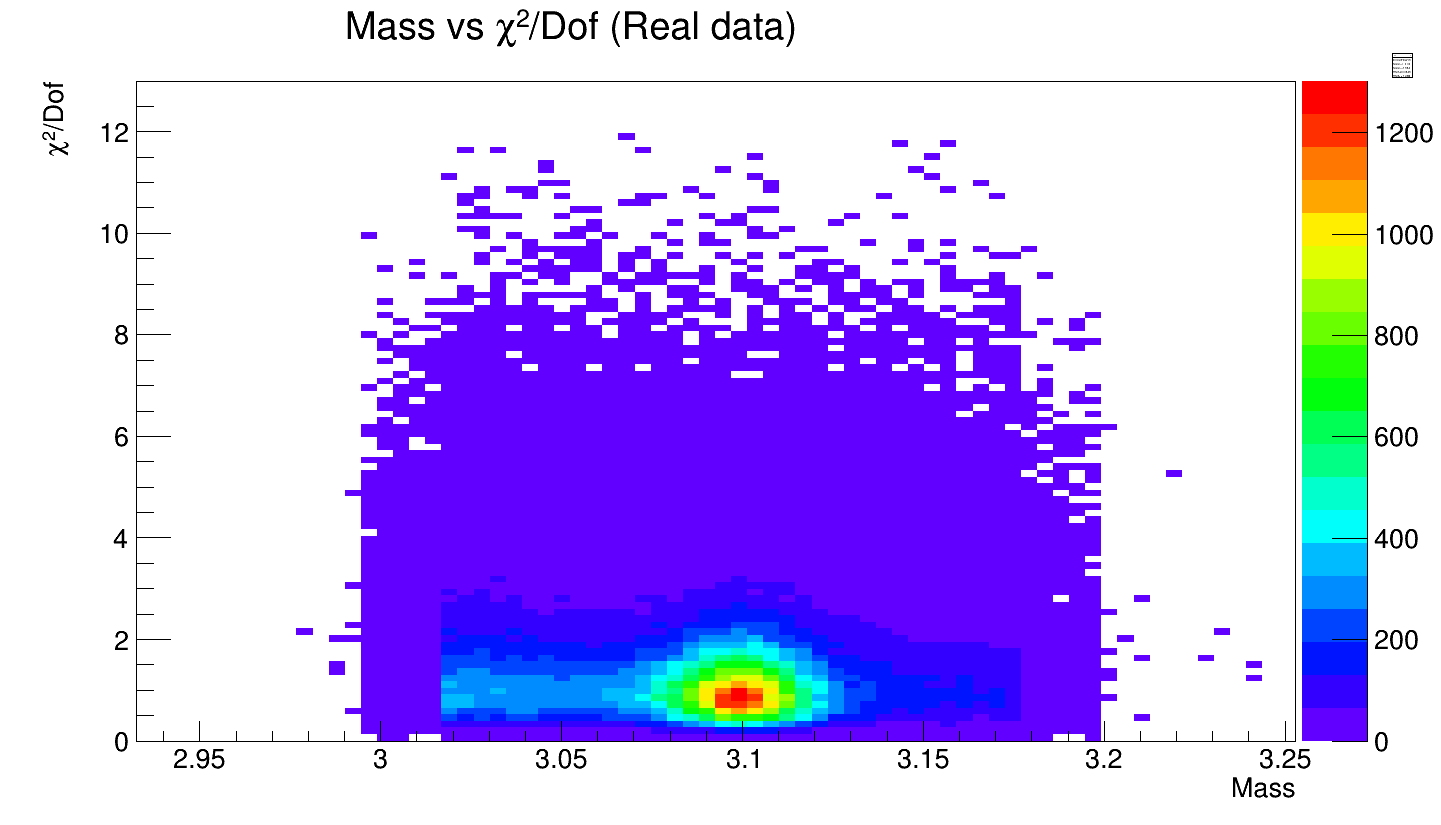
\includegraphics[width=\linewidth]{rozdzial6/JPsi_mass_chi2TT_data.png}
\end{minipage}

\vspace*{0.5cm} % (or whatever vertical separation you prefer)
\begin{minipage}[t]{0.5\textwidth}
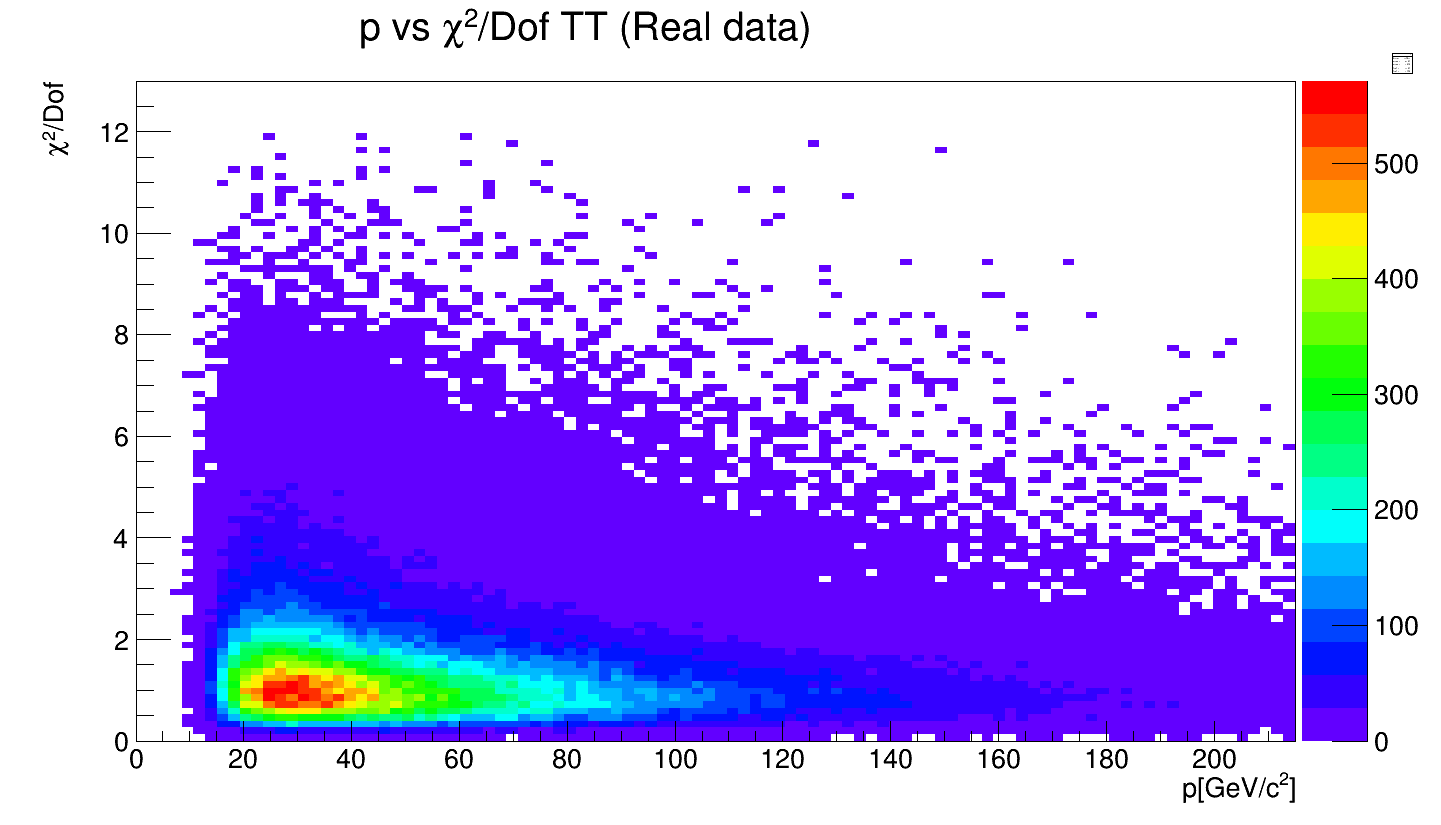
\includegraphics[width=\linewidth]{rozdzial6/JPsi_p_chi2TT_data.png}
\end{minipage}
\hspace{\fill}
\begin{minipage}[t]{0.5\textwidth}
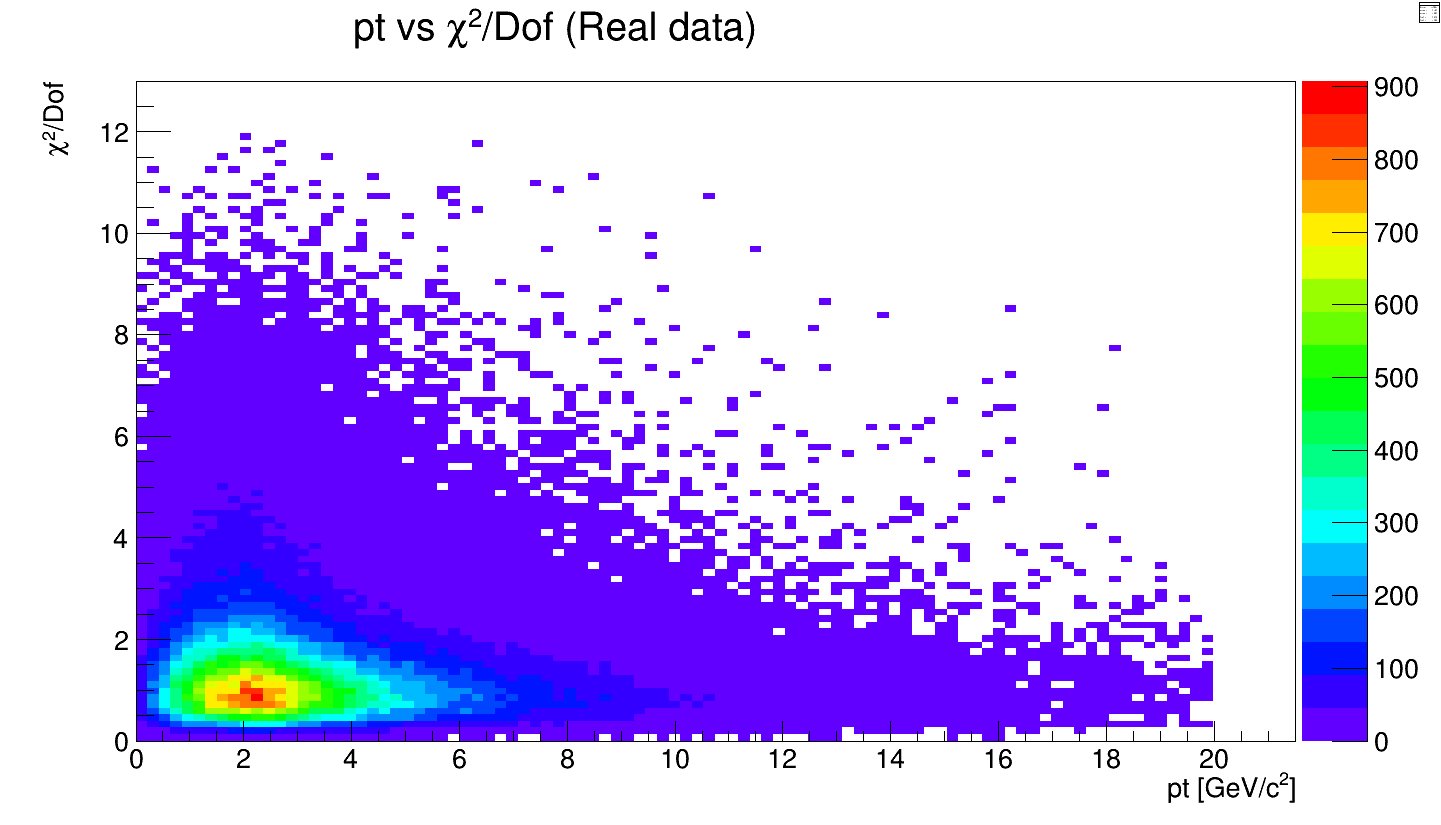
\includegraphics[width=\linewidth]{rozdzial6/JPsi_pt_chi2TT_data.png}
\end{minipage}
\caption{Korelacie pomiędzy $\chi^2_{TT}$  a (góra lewo) pseudorapidity, (góra prawo) masą niezmieniczą układu pionów oraz pędami całkowitym (dół lewo) oraz poprzecznym (dół lewo). Ślady pochodzą z rozpadu $J / \Psi$. Wykresy wykonano bazując na danych rzeczywistych, zebranych przez układ detekcyjny LHCb.} \label{corr_chi2JPsiTT_data}
\end{figure}


\section{Krytyka otrzymanych wyników}

Otrzymane wyniki, będące z całą pewnością interesujące i obrazujące problemy w dotyczące jakości rekonstrukcji śladów w eksperymencie LHCb niestety są wrażliwe na wielkość statystyki.   
Pierwszorzędnym celem kolejnych studiów nad tym efektami, które będą prowadzone przez autora, powinno być zwiększenie statystyki przypadków.  